
\documentclass[refcompress,eversion,noinfo]{ICTthesis}

%\usepackage{amssymb}
%\usepackage[thmmarks]{ntheorem}
\usepackage{amsmath}
\usepackage{amsthm}
\usepackage{tabularx}
\usepackage{longtable}
\usepackage{color}
\usepackage{colortbl}
\usepackage{graphicx}
\usepackage{subfigure}
\usepackage{epsfig}
\usepackage{enumerate}
\usepackage{multirow}
\usepackage{amsfonts}
\usepackage{algorithm}
\usepackage{algorithmicx}
\usepackage{algpseudocode}
\usepackage{tikz}
\usetikzlibrary{decorations.pathreplacing}
%\usepackage[margin=1.1in]{geometry}

\graphicspath{{figures/}}
%\linespread{1.3}

\definecolor{bkcolor1}{gray}{0.95}
\definecolor{bkcolor2}{gray}{0.85}
\newcommand{\bkcommand}[1]{\colorbox{bkcolor1}{$\mathtt{\backslash}$\texttt{#1}}}
\newcommand{\textgraph}[1]{\raisebox{-1ex}{\includegraphics[width=1.5em]{#1}}}

%\floatname{algorithm}{算法}
\renewcommand{\algorithmicrequire}{\textbf{Input:}} 
\renewcommand{\algorithmicensure}{\textbf{Output:}}

%\theoremsymbol{$\square$}
%\newtheorem*{proof}{证明}
\theoremstyle{plain}
%\theoremsymbol{}
%\theoremseparator{:}

\newtheorem{theorem}{定理}
\newtheorem{lemma}{引理}
\newtheorem{proposition}{命题}
\newtheorem{corollary}{推论}
\newtheorem{definition}{定义}

\newcommand{\upcite}[1]{\textsuperscript{\cite{#1}}}

\begin{document}
\ICTfrontmatter

\begin{abstract}

影响力最大化问题是在社交网络中选择$k$个种子以

\keywords{社会影响力, 小世界网络, 近似算法, 路由}

\end{abstract}

\begin{englishabstract}

Influence maximization is the problem of selecting $k$ nodes in a social network to maximize their influence spread.
The problem has been extensively studied but most work focuses on the submodular influence diffusion models.
In this paper, motivated by empirical evidences, we explore influence maximization in the non-submodular regime.
In particular, we study the general threshold model in which a fraction of nodes have non-submodular threshold
	functions, but their threshold functions are closely upper- and lower-bounded by some submodular
	functions (we call them $\varepsilon$-almost submodular).
We first show a strong hardness result: there is no $1/n^{\frac{\gamma}{c}}$ approximation for influence maximization (unless P = NP)
	for all networks with up to $n^{\gamma}$ $\varepsilon$-almost submodular nodes, where $\gamma$ in $(0,1)$ 
	and $c$ is parameter depending on $\varepsilon$.
We then provide constant approximation algorithms when the number of non-submodular nodes are constant.
Finally, we conduct experiments on a number of real-world datasets, and the results demonstrate that our approximation algorithms
	outperform other benchmark algorithms.

\englishkeywords{Social Influence, Small World Network, Approximation Algorithm, Routing}

\end{englishabstract}

\ICTmainmatter

\chapter{绪论}
二十一世纪互联网发展迅猛,人与人之间不再仅仅只能当面交流,电子邮件、电话和即时通讯软件让人们之间的沟通更迅捷。与此同时,社交网站也在兴起,积累了越来越多的用户。在社交网络中,信息传播得更快,在社交网络中的营销手段会比传统营销获得更大的收益,有一些相关学者开始关注社交网络中的信息传播现象。


\section{课题研究的背景与意义}
社交网络(Social network)是由许多节点构成的一种社会结构。节点通常是组织和个人,节点之间的连接代表社会个体之间的关系,经由这些社会关系,把从偶然相识的泛泛之交到紧密结合的家庭关系的各种人们或组织串连起来。“社交网络”的概念从心理学、社会学、人类学、数学、统计学、计算机科学等不同领域不断深化,形成了一套系统的理论、方法和技术。在21世纪,人们获取信息的途径不再局限于报纸、广播、电视和当面交谈,随着Facebook,Twitter和Weibo等社交工具的广泛应用,社交网络已经成为重要的信息传播工具。在社交网络上,人们通过添加好友和关注建立人与人之间的连接,通过发消息、短文章、分享连接进行交流。信息在社交网络上可以沿着人与人之间的连接很快传播,很多新闻、广告在社交网络上可以很快的覆盖到绝大多数用户,这相对于传统的媒体介质有很大的优势。在互联网时代,社交网络成为了重要的信息传播工具,利用社交网络进行产品或信息的推广是很有力的手段。在实际应用场景中,会有这样的案例,某公司准备发售一款新产品,想要在社交网络上做一些免费体验活动,希望免费体验的人可以把产品较好的口碑在朋友间扩散出去,最后达到产品推广的目的。随之产生了这样一个优化问题,给定了网络结构和信息传播的模型之后,如何选定k个人作为种子,使得这$k$个人最后影响的范围最大,这就是社会网络影响力最大化\cite{Kempe2003maximizing}。这个问题被证明是NP难的,而且因为社交网络的规模很大,暴力的枚举所有种子集合很不现实,设计高效的有近似比保证的算法是很有需求的。

社会网络影响力最大化在被Kempe, Kleinberg和Tardos\cite{Kempe2003maximizing}提出并公式化之后,已经在学术界引起了广泛的关注,近年来很多学者都在做相关研究,涉及到病毒营销、媒体广告和谣言传播等方向。很多学者提出了比较有效的算法\cite{Kempe2003maximizing,Leskovec2007celf,Chen2009efficient,chen2010sharpphard,tang2014newrrset},这些算法大部分是采用了独立级联(Independent Cascade)或者线性阈值(Linear Threshold)[1]的信息传播模型。在这两种传播模型下,影响力函数是次模(Submodular)的,这时候可以使用贪心策略得到1-1/e近似的算法。此外,在一个更一般的通用阈值(General Threshold)\cite{Kempe2003maximizing}传播模型下,每个用户的阈值函数(Threshold Function)不再是简单的把边的权值相加,而是一个集合函数。伯克利的学者Elchanan和Sebastien\cite{Mossel2007sub}证明了阈值函数是次模的时候整体的影响力函数也是次模的,也就意味着局部的次模性质会导致全局的影响力函数的次模性。

然而,在真实的社交网络中,非次模的影响力传播现象经常出现。Backstrom[6]研究了LiveJounral和DBLP两个大型的社交网络数据,他绘制了个体加入某个社区的意愿与她的已经加入该社区好友数量的关系图。论文的图中可以看到意愿曲线整体上是上凸的,但是在最开始几个点有明显的下移。杨洋[7]等人观测了另一个社交网络Flickr,他们主要观察人的情绪变化被他带有情绪的朋友的影响。他们指出人变快乐的可能性和已经快乐的好友数量是一个超线性关系,尤其是那些影响力比较大的朋友。这些结果都指出现有的基于独立级联或者线性阈值模型的算法在真实的社会网络种可能并不能使用。很多非次模的传播模型已经被证明很难近似,像谣言和疾病的传播,需要社交网络中的个体在被影响邻居的数量超过某个阈值的时候才会被影响,这种模型也是通用阈值模型的变种,被称作固定阈值模型(Fixed Threshold Model)。在固定阈值模型下,社交网络影响力最大化问题是NP-hard的,而且有很强的不可近似性[1]。与此同时,如果考虑寻找能达到给定影响力目标的最小种子集合问题,也就是社会影响力最小化种子集合问题,陈宁也证明了这个问题也很难被近似[8]。学者们倾向于相信是次模性质帮助我们在社会影响力最大化问题中找到了比较好的近似算法。但是我们可以使用次模性质到什么程度呢?如果影响力传播过程仅仅是稍微偏离了次模性质,那么是否还有可能仍然设计一个近似比足够好的算法呢?这些问题现在仍然是需要解决的。

与此同时,固定阈值模型下的问题还有一些仍未被探索,前面说到的影响力传播,实际上只关心最后影响的人的数量,而不关心传播的时间和步数。考虑给定种子和目标节点的情况下,在不知道整体网络结构时,如何才能通过影响最少的人而影响目标?其实可以规定一个时间片只能影响一个人,问题就变成了社会网络里面,在固定阈值模型下,从给定的种子到目标点需要经过多少步跳转或者多少个时间片。这就是从另一个角度来研究社会影响力,从影响力传播的时间而不是影响的范围。此外,这里研究的是路由现象,就像IP包在路由网络里转发一样,IP包只知道最后的目的地,并不知道每一步应该具体怎么转发,也不能在每一个路由器群发,只能一步一步的跳转。我们研究的就是在社交网络里面的路由现象,跟传统路由的区别有两个,一个是社交网络的结构,没有路由表;另一个是每个节点被影响的邻居超过一定阈值时才能被影响到。在文章里,称类似IP包跳转的现象为简单路由,把影响需要阈值的路由为复杂路由。

社交网络是一个小世界网络,人与人之间的最短路很短。二十世纪60年代,美国哈佛大学社会心理学家斯坦利·米尔格伦(Stanley Milgram)做了一个连锁信实验[9]。他将一些信件交给自愿的参加者,要求他们通过自己的熟人将信传到信封上指明的收信人手里,他发现,294封信件中有64封最终送到了目标人物手中。而在成功传递的信件中,平均只需要5次转发,就能够到达目标。也就是说,在社会网络中,任意两个人之间的“距离”是6。这就是所谓的“六度分隔”理论(Six Degrees of Separation)。尽管他的实验有不少缺陷,但这个现象引起了学界的注意。小世界网络就是对这种现象(也称为小世界现象)的数学描述。用数学中图论的语言来说,小世界网络就是一个由大量节点构成的图,其中任意两点之间的平均路径长度比节点数量小得多。除了社会网络以外,小世界网络的例子在生物学、物理学、计算机科学等领域也有出现。许多现实中的图可以由小世界网络作为模型。万维网、公路交通网、脑神经网络和基因网络都呈现小世界网络的特征。本文采用经典的Kleinberg网络[10],这是一个基于二维网格的小世界网络,网格的边被称为人与人之间的强链接,而同时每个节点会发出若干条随机的弱连接。Kleinberg指出当模型的参数α等于网格的维度时,贪心路由算法有很高的效率。这里的贪心路由算法是指在每一步,当前节点把消息传递给他的邻居里面距离目标节点曼哈顿距离最小的节点。这个路由算法的需要的跳转数也符合之前Milgram的实验结果,从理论上支持了小世界现象。Kleinberg进一步指出当模型的参数α不等于网格的维度时,所有的路由算法都不能很快地把信件送达到目标手中。本文关注的是小世界网络中复杂路由的速度,复杂路由每一步激活的过程就是固定阈值模型,也是通用阈值模型范畴下的子问题。


\section{国内外研究现状}
自从基于BoW的图像检索框架\cite{sivic2003video}被提出以来,国内外学者对BoW中的几何校验问题就从未终止。针对BoW框架的几何校验基本可以分为两类,即检索后校验和检索时校验。检索后校验是指在进行正常的BoW检索之后,基于查询图片和匹配图片中特征点的几何一致性,对检索结果进行重新排序。检索后校验只考虑匹配点的几何关系,并且一般情况下,后校验的算法时间复杂度较高,只能对初排序结果的top N进行几何校验。检索时校验是指在进行BoW检索过程中进行几何校验,所以这种方法会考虑每对特征点之间的几何一致性。这就要求必须在进行检索之前将一些额外的有关于几何关系的信息融入到BoW向量中或倒排表内。一般情况下,检索时校验不会进行非常严格的几何校验,但是具有较高的检索效率。

\cite{sivic2003video}使用了一种相对简单的几何校验方案,称为空间一致性(Spatial Consistency)校验。这种校验考虑每个匹配点(局部特征点或区域)最近邻的匹配情况。具有空间一致性的点其最近邻的匹配点也应该在同一块区域内。这种方法只考虑了特征点在图片中相对位置关系的一致性。可以看出空间一致性检验是一种后校验方案。

利用RANSAC算法进行空间校验可以得到最好的几何校验效果,因为它要求很高的几何变换的一致性。首先定义匹配点之间变换矩阵,一般会考虑平移、旋转和尺度变换;然后计算每对匹配点之间的变换矩阵,并基于RANSAC算法得到最优的变化矩阵;最后根据这个变换矩阵,测试每对匹配点,符合这个变换的的点对被称为“inliers”,“inliers”数决定图片最终的相似度。\cite{philbin2007object}基于上述思想提出了Fast Spatial Matching(FSM)算法。由于FSM也是一种后校验的算法,FSM具有较高的计算复杂度,并且只能对Top N的检索结果进行校验,不能保证高召回率。\cite{Zhong2015Fast}对FSM做出改进并提出Direct Spatial Matching(DSM)。DSM直接计算尺度的变换,相比于其他基于RANSAC的算法,DSM需要更少的校验时间。

由于后校验的方法计算复杂度高、低召回率等问题,检索时校验同样得到人们的关注。这其中最经典的方法是基于空间金字塔(Spatial Pyramid)的几何校验算法。\cite{lazebnik2006beyond}和\cite{Cao2010Spatial}都是基于某种规则将一副图像分成若干区域,然后为每个区域生成一个BoW向量,最后将这些BoW向量连接到一起生成整幅图像的BoW向量。\cite{Cao2010Spatial}提出Spatial Bag-of-Features是\cite{lazebnik2006beyond}中Spatial Pyramid Matching的一般形式并且Spatial Bag-of-Features可以处理目标的基本变换,例如平移、旋转和尺度变化等。

近些年,CNN(Convolutional Neural Networks)在计算机视觉领域取得了巨大的成功,例如图像分类\cite{krizhevsky2012imagenet}、目标检测\cite{Girshick2014Rich}\cite{girshick2015fast}\cite{ren2015faster}、人脸识别,也包括图像检索\cite{babenko2014neural}。对于图像检索问题,一般是使用训练好的模型(同时可能会在某些数据集上进行fine-tune)提取图片的全局特征(网络某一层的输出),然后进行相似度的计算并排序。不同于传统的BoW检索框架,基于CNN的检索框架不考虑图片的旋转和尺度变化,而完全依赖于模型的能力和大规模的训练数据。在实际检索场景下,图片旋转是常见问题。现有网络一般使用Max Pooling操作,可以一定程度上应对旋转问题。

可以看到,国际上对于图像检索中几何校验的研究正呈现百花齐放的状态,研究人员从不同角度对几何校验进行了多方面的研究,形成了不同的算法与思路,这也恰好说明了人们对于显著性区域检测这一课题还处于探索研究阶段,并没有形成最优的解决方案,还存在多方面的问题亟待解决。



\section{本文所做的工作}
本文针对目前检索框架(包括BoW检索框架和CNN检索框架)中存在的问题,在Word Spatial Arrangement(WSA)\cite{penatti2014visual}基础上做出改进,提出Region Property Arrangement(RSA)空间校验算法。并且训练了学习图片主方向的CNN网络Main Orientation Net来解决CNN检索框架中图片旋转的问题。主要工作与成果如下:

\begin{enumerate}
\item  通过对WSA和其他空间校验算法的深入研究,提出了RSA空间校验算法。RSA方法首次提出了Region Property Space(RPS)的概念,并将图片中的特征区域(interest region)映射为RPS中的一个点。传统的空间校验算法只考虑匹配点对之间尺度、角度的相对变化,而RSA可以分析一副图片所有特征区域属性的分布规律,并将这种分布编码到BoW向量中,可以在检索过程中完成几何校验。RSA算法可以显著提高BoW检索的性能,在Holidays、Paris和Oxford数据库上达到了state-of-the-art的检索性能,同时不会增加计算和存储的负担。
\item  通过对RPS中点的分布进行深入的研究,我们发现RPS中点的分布具有很强的规律性,这种规律性在图片位置空间(基于特征点在图片上出现的位置)所不具备的。通过分析,我们在RPS的基础上提出了Spatial Weighting(SpW)。SpW可以解决图像检索中的burstniess\cite{jegou2009burstiness}的问题。并且,基于RPS中点的分布特性,我们提出了计算RSA的快速算法,比暴力算法快2到3倍。
\item 为了应对图像检索中图片旋转的问题,我们提出了MONet(Main Orientation Net)。由于图片主方向包含了图片的语义信息,传统的方法无法得到(只能得到某个区域的梯度方向)。借助深度学习方案,MONet很好的解决了查询图像可以旋转的问题,提高的检索的准确率。
\end{enumerate}

\section{论文组织结构}
本文分为五章,主要结构和内容如下:

第一章首先阐述了显著几何校验的研究背景和意义,接着介绍了该方向的国内外研究现状以及存在的问题,最后概述了本文所做的工作和论文的组织结构。

第二章介绍显几何校验测的基础特征与算法,并分类探讨了目前国际上各类主流算法的思路与不足。基于此,制定了本文的研究思路与框架。

第三章介绍Region Similarity Arrangement和Spatial Weighting算法,并通过详细的实验对比,全面评测了该算法的性能。

第四章介绍 Main Orientation Net,并将该网络应用到BoW和CNN检索框架中,对算法性能进行了全面评估。

最后一章对全文进行了总结,同时展望未来的研究工作。


\chapter{小世界网络及影响力传播基础}
在本章中,首先介绍Kleinberg小世界网络模型和影响力传播模型,
然后介绍常见的影响力传播模型,
最后介绍了影响力最大化算法的相关工作。

\section{Kleinberg小世界模型}\label{sec:kleinberg}
Kleinberg的小世界模型是一个由$n$个节点的集合$V$生成的随机图。
$n$个节点分布在一个$\sqrt{n} \times \sqrt{n}$的二维网格上\cite{Kleinberg2000small},为了方便,
我们把网格的上边界和下边界连接起来,同时也把网格的左边界和右边界连接起来。
这样二维网格就变成了“环面”,网格中每个节点的位置都是对称的。
网格上两个节点$u$和$v$之间的曼哈顿距离(Manhattan distance)$|uv|$是
在网格上$u$到$v$的最短路径的长度。

这个随机图上有两种类型的边:{\it 强连接}和{\it 弱连接}。
强连接是任意两个曼哈顿距离不超过$p$的节点之间生成的无向边,这里$p \geq 1$是一个模型的常数。
弱连接指连接节点$u$和网格上可能相距较远的节点$v$之间的随机边。
每个节点$u$会有$q$条互相独立的弱连接边,$u$的第$i$条弱连接边以$v$为终点的概率
正比于$1/{|uv|}^\alpha$,$\alpha\geq 0$是小世界模型的参数。
我们用$1/{|uv|}^\alpha$乘以归一化因子$\mathcal{Z} = 1/\sum_{v\in V}|uv|^{-\alpha}$(在环形网格上,这个值对于任意的节点 $u\in V$都相等),这样就得到了弱连接的概率分布函数。
最初Kleinberg描述的网络模型\cite{Kleinberg2000small}中,$u$到$v$之间的弱连接被认为是有向边,这样的网络被称为{\it 有向Kleinberg小世界网络模型}。
而有些研究工作\cite{Ghasemiesfeh2013complex}中弱连接被认为是无向的,这样的网络被称为{\it 无向Kleinberg小世界网络模型}。
两个模型在本文中都被讨论了,在分析复杂传染病的传播时,我们为了和以前的工作保持一致,
采用无向Kleinberg小世界网络模型。
分析复杂传染病的路由时,我们使用有向Kleinberg小世界网络模型。

\section{影响力传播模型}
社交网络被定义为一个有向图$G=(V,E)$,其中$V$是所有节点的集合,代表着网络中的个体,$E\subseteq V \times V$是有向边的集合。
$E$是网络中的关注或者粉丝关系,每条边也会有权值,权值代表着两个人的关系密切程度或者影响程度。
因为$G$是有向图,对于一个节点$v$,我们用$N^+(v)$表示所有$v$指向的节点集合,用$N^-(v)$表示所有指向$v$的节点集合,也就是$v$的出邻居(out-neighbours)和入邻居(in-neighbours)集合。
网络中的节点都有两种状态:{\it 未激活}(inactive)和{\it 激活}(activated)。
节点可以从未感染状态转变为感染状态,但是不能反方向转变,例如不能从已感染的状态变成未感染状态。
传播的过程可以用离散的时间步骤$0,1,2,\ldots$来描述。
在社交网络模型下,影响力传播被定义为一些疾病、信息或者想法在社交网络中沿着用户之间的有向边进行扩散。
对于一次传播过程,初始状态节点都是未激活的,选定图中的一些节点,把他们的状态设定为激活。
然后每一个时间片,按照设定的传播模型逐渐去尝试激活图未激活中的节点。
如果当前时间片没有新的节点被激活为止,传播过程结束。
接下来本文介绍常见的影响力传播模型。


\subsection{独立级联模型}
\begin{figure}[h]
	\centering
	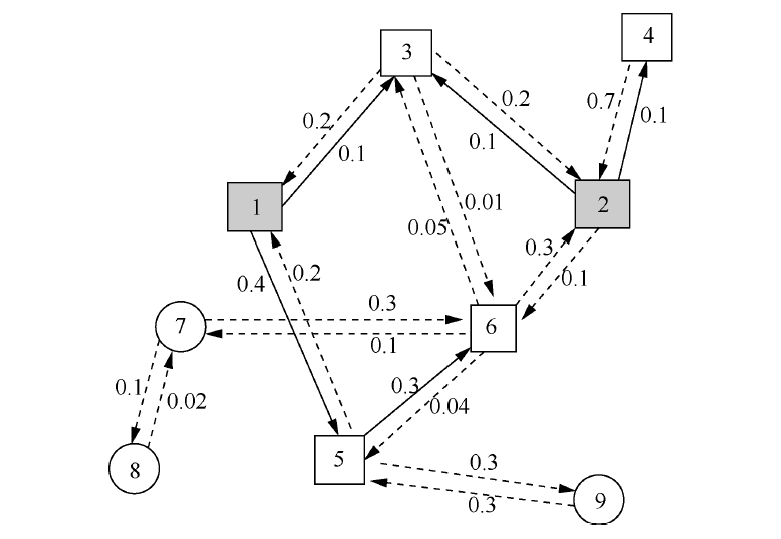
\includegraphics[width=\textwidth]{independent_cascade.png}
	\caption{独立级联模型示意}\label{fig:independent_cascade}
\end{figure}
独立级联模型(Independent Cascade Model)在03年被Kempe等人\cite{Kempe2003maximizing}提出,
在独立级联模型中,每条有向边$(u,v) \in E$都有一个概率值$p(u,v) \in [0,1]$代表着$v$被$u$影响的概率。
传播是随着离散时间片$t$增加而扩散的,定义$S_t$为到时间片$t$时刻为止被激活的节点的集合,定义$S_{-1}=\emptyset$。
在$t=0$时刻,选定$k$个节点$S_0$作为种子并把他们置为激活状态。
对于任意的$t\geq 1$时刻,每一个在$t-1$时刻激活的节点$v \in S_{t-1} \setminus S_{t-2}$都会对其所指向的未激活节点
$u \in N^+(u) \setminus S_{t}$进行一次激活尝试,成功激活$u$的概率是$p(v,u)$,不同节点之间的激活尝试相互独立。
如果节点$u$在某次激活尝试中被激活,则$u$在$t$时刻被激活。
如果$S_{t-1} \setminus S_{t-2}$中所有节点对$u$的尝试都失败,则$u$在$t$时刻未被激活。
当某一时刻没有节点被激活时,传播终止。

图\ref{fig:independent_cascade}给出了独立级联模型下的一次传播过程,图中的虚线边表示一次失败的激活尝试,实线表示成功的激活尝试。
在$t=0$时刻节点1和节点2被选为种子,在$t=1$的时刻,节点1和节点2成功激活了节点3、4、5,节点2对节点6的激活尝试失败。
在$t=2$时刻节点5成功激活了节点6,节点3和4发出的尝试激活失败。
在$t=3$时刻节点6没有激活任何节点,传播过程终止,最后被影响的节点集合是$\{1,2,3,4,5,6\}$。

\subsection{线性阈值模型}
独立级联模型(Linear Threshold Model)\cite{Kempe2003maximizing}描述的传播过程中,节点对节点的作用是互相独立的,而且每个节点只需要一次成功的激活尝试就能被激活。
而在有些场景中,一个节点的激活需要多个节点的共同作用,像购物或者接受新商品等。
为了描述类似举要多个节点累计作用才能激活的场景,线性阈值模型被提出来。

在现行与之模型中,每条有向边$(u,v) \in E$都被赋予了一个权重$w(u,v)$,对于每个节点来说,所有指向它的边权重之和不超过$1$。
也就是$\sum_{u \in N^-(u)} w(u,v) \leq 1$。
每个节点$v$还有自己的阈值$\theta_v \in [0,1]$,在传播开始前,每个节点独立的在$[0,1]$中依据均匀分布选择自己的阈值。
在每个时间节点$t \geq 1$,对于所有还没被激活的节点$v \in V \setminus S_{t-1}$,
如果由已激活节点发出的指向$v$的的有向边权重之和大于$v$的阈值,也就是$\sum_{u \in N^-(u) \cap S_{t-1}} w(u,v) \geq \theta_v$,
则$v$会在$t$时刻被激活,否则停留在未激活状态。
同样,当在某一时刻没有新节点被激活时,传播停止。

\subsection{通用级联模型}
独立级联模型的假设过强,于是Kempe\cite{Kempe2003maximizing}提出了通用级联模型(General Cascade Model),
这是独立级联模型的一般形式。
对于通用级联模型,每个节点$v$有个激活函数$p_v(u,S):N^-(v) \times 2^{N^-(v)} \to [0,1]$,
这里$S \subset N^-(v)$并且$u \in N^-(v) \setminus S$。
传播过程整体和独立级联模型一致,
在$t=0$时刻选定种子节点后,在$t \geq 1$的时间片,
对于尚未激活的节点$v \not\in S_{t-1}$,把$v$刚刚激活的的入邻居$N^-(v) \cap (S_{t-1}\setminus S_{t-2})$按照$u_1,u_2,\dots,u_{\ell}$排列,
依据这个顺序依次尝试激活节点$v$。
如果$u_1,u_2,\dots,u_{i-1}$没有成功激活$v$,则令$S = (N^-(v) \cap S_{t-2}) \cup \{u_1,u_2,\dots,u_{i-1}\}$
然后$u_{i}$以$p_v(u_i,S)$的概率尝试激活$v$。
在通用级联模型中,$p_v(u,S)$满足顺序无关性质,也就是最终$u_1,u_2,\dots,u_{\ell}$尝试激活$v$之后$v$被激活的概率
与这$\ell$次尝试的顺序无关,只与尝试激活的节点集合有关。
注意到独立级联模型是通用级联模型的特例,只需要令$p_v(u,S)$恒等于$p(u,v)$即可。


\subsection{通用阈值模型}
在通用阈值模型中(General Threshold Model),每个节点$v$有一个阈值函数$f_v:2^{N^-(v)} \to [0,1]$。
阈值函数$f_v$是单调非减(monotone)而且$f_v(\emptyset)=0$。
和线性阈值模型相同,在传播开始前,每个节点独立的在$[0,1]$中依据均匀分布选择自己的阈值。
然后在接下来的每一时刻$t\geq 1$,对于$v \not\in S_{t-1}$,
如果$f_v(S_{t-1} \cap N^-(v)) \geq \theta_v$,
节点$v$被激活,否则节点$v$保持未激活状态。

%线性阈值模型是通用阈值模型的特例,只需要令$f_v(S) = \sum_{u\in S}w(u,v)$。
通用阈值模型和通用级联模型也是等价的,给定阈值函数$f_v$,可以得到激活函数
$p_v(u,S) = \frac{f_v(S \cup \{u\}) - f_v(S)}{1-f_v(S)}$。
给定激活函数$p_v$,同样可以得到对应的通用阈值模型的阈值函数
$f_v(S) = 1 - \Pi_{i=1}^{\ell}(1-p_v(u_i, \{u_1,u_2,\dots,u_{i-1}\}))$。


\section{影响力最大化问题}
在一个$n$个节点的图中,给定影响力传播模型,最多经过$n-1$步,传播就会结束。
我们称以$S_0$为种子集合最终传播停止时被影响的节点集合是$\Phi(S_0)$。
$\Phi(S_0)$是一个依赖于影响力传播过程的随机集合。
影响力最大化问题就是在给定种子数量选择合适的种子集合的情况下最大化$\Phi(S_0)$的期望大小。
我们定义$\sigma(S_0) = \mathbb{E}(\Phi(S_0))$,$\sigma(\cdot)$就被称作为{\it 影响力函数}。
通常所研究的种子集合大小不超过$k$的影响力最大化问题可以公式化为$S^* = \mathrm{argmax}_{S \in V, |S|=k} \sigma(S)$,
$S^*$为最优解集合。
通常选用的影响力模型是独立级联模型或者线性阈值模型,近些年来也有很多基于这两个传播模型的影响力最大化算法被提出。

影响力最大化本质上描述了社交网络中的营销(Social marketing)问题,
有新的产品或者广告发布时,希望选择人试用并转发消息,然后口口相传最后扩散到很多人。
商家最后的目的就是希望可以遭到影响力最大的用户集合使得最终扩散的范围最大,这也就是影响力最大化的目标。
影响力最大化问题是社交网络中营销问题的抽象,研究影响力最大化问题对于商家试用品和广告的投放有很大帮助。
下面介绍一下影响力最大化问题的常见算法。

\subsection{贪心算法}
影响力最大化问题的复杂度很高,至少比集合覆盖最大化(Max Set Cover)问题要难,而集合覆盖最大化问题是NP-Hard的。
但是影响力函数$\sigma(\cdot)$在独立级联模型和线性阈值模型下被证明是次模的\cite{Kempe2003maximizing}。
次模函数是定义在集合函数上的,对于一个集合函数$f:2^V \to \mathbb{R}$,
如果对于任意的输入集合$S \subseteq T \subseteq V$和元素$u \in V \setminus T$都有
$f(S \cup \{u\}) - f(S) \geq f(T \cup \{u\}) - f(T)$,
则称函数$f$满足次模(submodular)性质。
次模性质本质上是边际效益递减,同样加入一个元素$u$,$f(T)$函数值的提升不如$f(S)$的提升大。
如果对于输入$S \subseteq T \subseteq V$,$f$函数还满足$f(S) \leq f(T)$,则称函数$f$是单调非减的。
对于单调非减和次模的函数$f$,贪心算法可以做到$1-\frac{1}{e}$的近似比。
对于影响力最大化问题,由于影响力函数$\sigma(\cdot)$是单调和次模的,可以调用贪心算法解决。
然而每一步$\sigma(S)$的计算是$\#$P-Hard的,不能精确求解。
通常采用蒙特卡洛模拟方法来估算影响力,随机模拟10000次传播过程,取被激活节点个数的期望作为影响力。
由于蒙特卡罗模拟是近似得到影响力大小,贪心算法最后可以取得$1-\frac{1}{e}-\varepsilon$的近似比。
蒙特卡洛贪心算法执行过程如Algorithm \ref{alg:mc_greed}所示。

\begin{algorithm}[h]
	\caption{\textbf{MC-Greedy(G,k)}: Monte Carlo greedy for influence maximization.}
	\label{alg:mc_greed} 
	\begin{algorithmic}[1]
		\Require $G$: social graph of IC or LT model, $k$: budget of seeds.
		\Ensure selected seed set $S$.
		\State Initialize $S = \emptyset$
		\For {$i=1$ to $k$}
			\State $v = \mathrm{argmax}_{u \in V \setminus S}$ \Call{MC-Spread}{$S \cup \{u\}, G$}
			\State $S = S \cup \{u\}$
		\EndFor
		\State \Return $S$
		\Function{MC-Spread}{$S$, $G$}
			\State $count=0$
			\For {$j=1$ to $R$}
				\State simulate diffusion process on graph $G$ with seed set $S$
				\State $n\_spread \gets$ the number of active nodes
				\State $count = count + n\_spread$
			\EndFor
			\State \Return $count/R$
		\EndFunction
	\end{algorithmic} 
\end{algorithm}

\subsection{CELF算法}
暴力的贪心算法时间复杂度很高,对于$k$个种子的影响力最大化问题,需要迭代$k$轮,每一轮需要便利每一个种子,利用蒙特卡洛模拟估计影响力大小。
最终需要的时间复杂度为$O(Rknm)$,$R$是蒙特卡洛模拟需要的传播模拟次数。对于几万个节点的图,贪心算法的运行时间可能就需要几周。
Leskovec等人\cite{Leskovec2007celf}基于次模问题优化中的lazy evaluation方法,优化了暴力的贪心算法,得到了近700倍的算法性能提升。
定义函数的差分为$\Delta_u f(S) = f(S \cup \{u\}) - f(S)$,其中$u \not\int S$。
对于单调次模函数$f$和集合$S \subseteq T \subseteq V$来说,有$\Delta_u f(S) \geq \Delta_u f(T)$。
在蒙特卡洛贪心算法中,每一轮都需要计算每个节点$v$的$\Delta_v f(S)$然后选出提升最大的节点加入$S$。
设$S_i$为第$i$轮为止选择到的种子节点集合,如果在第$i$轮算法运行中,发现存在节点$u,v \not\in S_{i-1}$,而且$\Delta_u f(S_{i-2}) \leq \Delta_v f(S_{i-1})$。
那么由次模性质可以得到$u$在第$i$轮的提升一定会小于$v$,所以不会被选为种子,在第$i$轮$u$的影响力提升就没有必要再计算。
所以加入一个结构存储之前计算的影响力提升,可以减少对影响力的重复估算,极大提升算法效率。
CELF算法就是利用这个思想,通过优先队列实现。

\begin{algorithm}[h]
	\caption{\textbf{CELF(G,k)}: accelerated greedy algorithm with lazy evaluation.}
	\label{alg:celf} 
	\begin{algorithmic}[1]
		\Require $G$: social graph of IC or LT model, $k$: budget of seeds.
		\Ensure selected seed set $S$.
		\State Initialize $S = \emptyset$, priority queue $Q = \emptyset$
		\ForAll {$v$ in V}
			\State $v.margin \gets$ \Call{MC-Spread}{$\{v\}, G$}
			\State $v.iteration = 1$
			\State insert element $v$ into $Q$ with $v.margin$ as the key
		\EndFor
		\State $iteration = 1, spread = 0$
		\While{$iteration \leq k$}
			\State extract top (max) element $v$ of $Q$
			\If{$v.iteration == iteration$}
				\State $S = S \cup \{u\}$
				\State $iteration = iteration+1$
				\State $spread = spread + v.margin$
			\Else
				\State $v.margin \gets$ \Call{MC-Spread}{$S \cup \{v\}, G$} - $spread$
				\State re-insert $v$ into $Q$
			\EndIf
		\EndWhile
		\State \Return $S$
	\end{algorithmic} 
\end{algorithm}

\subsection{PMIA算法}
MC-Greedy算法和CELF算法还是通过蒙特卡洛模拟来估算集合的影响力大小。陈卫等人提出了一个启发式算法,近似的估算影响力,再次提升了算法的性能,同时算法的效果能够媲美贪心算法。
PMIA算法\cite{chen2010sharpphard}中,利用比较容易计算的树状图来避免了蒙特卡洛模拟。
核心子算法是Maximum Influence Arborescence(MIA),PMIA算法对于每一个节点$v$构建了以$v$为根的局部树状结构,
然后在局部的树状结构上可以用动态规划高效计算影响力。
因为影响力传播衰减很快,而且估算整体的影响力很难,局部树状结构也是合理的。
PMIA算法同时也根据树状结构设计了线性更新影响力提升值的方法,在加入新的种子节点后很快更新每个节点的影响力。
原算法的整体过程比较复杂,由多个子算法构成,这里不再赘述。

\subsection{TIM算法}
基于蒙特卡洛模拟的贪心算法速度较慢,启发式算法速度较快但是没有理论的近似比保证。
Borgs等人\cite{borgs2014rrset}在14年提出了基于逆向可达集合(Reverse Reachable Set)的近线性算法,同时也有基于最大集合覆盖的$1-\frac{1}{e}$的近似比保证。
算法的核心思想是做逆向蒙特卡洛模拟,把图中每条有向边反向,沿着反向的边做传播。
算法会随机的选择图中的节点$v$,然后以$v$为根节点做反向蒙特卡洛模拟,传播过程中激活的节点称为$v$的逆向可达集合,多次模拟得到多个逆向可达集合。
Borgs等人证明了,给定种子集合$S$,$v$被激活的概率就是$S$和$v$的逆向可达集合有交集的概率。
因此可以随机从途中选择节点,产生逆向可达集合,多次实验之后生成很多逆向可达集合。
给定一个种子集合,影响力大小正比于种子集合与多少个多逆向可达集合有交集,这就转变为最大集合覆盖问题,可以用贪心很快求解。
随后Tang等人\cite{tang2014newrrset}工程上实现了这个算法(TIM算法),并测试了算法在上亿节点的效果和运行时间。该算法已经能处理Twitter这种级别的社交网络。
在求解最大覆盖问题时,依据逆向可达集合简历倒排索引,维护每个节点覆盖的逆向可达集合,每次贪心的选择覆盖最多逆向可达集合的节点加入种子节点。

\begin{algorithm}[h]
	\caption{\textbf{TIM(G,k)}: Two-phase Influence Maximization.}
	\label{alg:tim} 
	\begin{algorithmic}[1]
		\Require $G$: social graph of IC or LT model, $k$: budget of seeds.
		\Ensure selected seed set $S$.
		\State Initialize $S = \emptyset$, $\mathcal{R} = \emptyset$
		\State compute the the number of RRsets needed $\theta$
		\For {$i=1$ to $\theta$}
			\State randomly pick a node $v$ from $V$
			\State generate RRset $R_v$ for $v$
			\State insert $R_v$ into $\mathcal{R}$
		\EndFor
		\State build reverse index $Idx$ of $\mathcal{R}$
		\For {$i=1$ to $k$}
			\State fetch $v$ that has max degree from $Idx$
			\State insert $v$ into $S$
			\State update $Idx$
		\EndFor
		\State \Return $S$
	\end{algorithmic} 
\end{algorithm}

\section{本章小结}
本章主要介绍了本文使用的Kleinberg小世界模型以及影响力传播模型和影响力最大化算法等概念,并给出了精确的数学定义。
2.1节介绍了Kleinberg的小世界模型,主要分析了弱连接的生成方式。
2.2节介绍了影响力传播模型,重点介绍了线性阈值模型和独立级联模型以及他们的通用形式。
2.3节介绍了基于线性阈值模型或者独立级联模型和影响力最大化,影响力最大化算法在近些年来被许多学者研究,很多近似算法和启发式算法被提出。




\chapter{非次模影响力传播模型}
上一章介绍了影响力最大化问题的发展情况和现有算法。
但是这些算法都是基于次模的影响力传播模型,而且在设计算法的过程中大多也利用了次模的性质。
在本章,我们会介绍非次模模型,本文的研究也是基于所提出的非次模模型。

\section{$\varepsilon$-次模逼近函数}
通用阈值模型是影响力最大化问题中最重要的模型之一。
通常情况下,我们关注阈值函数(threshold function)的两个性质——次模性质(submodularity)和超模性质(supermodularity)。
次模性质可以被理解为在向种子集合添加新节点时,现有种子集合越大,获得的收益越小,也就是边际收益递减。
与之相反,超模性质是边际效益递增。
对于通用阈值模型来说,阈值函数的次模性质是贪心算法近似比的保证\cite{Mossel2007sub},
在这篇论文里,我们想要研究阈值函数是近次模函数的模型,这个函数被定义为$\varepsilon$-次模逼近函数($\varepsilon$-almost submodular function)。
接下来我们给出次模,超模和$\varepsilon$-次模逼近函数的精确定义。

\begin{definition}[次模 (Submodular)]
对于一个定义在集合上的函数$f:2^V \to \mathbb{R}$,
如果对于$V$的任意子集$S \subseteq T \subseteq V$和点$v \not\in T$都有
$f(S \cup \{v\}) - f(S) \geq f(T \cup \{v\}) - f(T)$,
则称$f$为次模函数。
\end{definition}

\begin{definition}[超模 (Supermodular)]
对于一个定义在集合上的函数$f:2^V \to \mathbb{R}$,
如果对于$V$的任意子集$S \subseteq T \subseteq V$和点$v \not\in T$都有
$f(S \cup \{v\}) - f(S) \leq f(T \cup \{v\}) - f(T)$,
则称$f$为次模函数。
\end{definition}

\begin{definition}[$\varepsilon$-次模逼近 ($\varepsilon$-Almost Submodular)]
对于一个定义在集合上的函数$f:2^V \to \mathbb{R}$,
如果存在一个同样定义在$2^V$上的次模函数$f^{sub}$和一个正数$\varepsilon<1$,
对于任意的$S \subseteq V$都有$f^{sub}(S) \geq f(S) \geq (1-\varepsilon)f^{sub}(S)$,
则称$f$为$\varepsilon$-次模逼近函数。
\end{definition}

本文只讨论有向图上的影响力传播,对于阈值函数$f$,如果函数值只依赖于输入集合的大小,我们可以简写为$f_v(S) = f_v(|S|)$。
$\varepsilon$-次模逼近函数描述了一类很接近次模但又不是次模的函数,直观上看$\varepsilon$-次模逼近函数的性质会和次模函数很接近。
本文主要研究非次模问题,在后续章节以$\varepsilon$-次模逼近函数为切入口,会讨论在阈值函数为$\varepsilon$-次模逼近函数时,影响力最大化问题能能否被近似。
$\varepsilon$-次模逼近函数在现实生活中也是有意义的,现实网络中很多影响传播过程都被观测到有非次模的现象。
Backstrom\cite{backstrom2006group}等人研究了LiveJounral和DBLP两个大型的社交网络数据,
他们把用户加入LiveJounral社区的概率看作已经加入社区用户的数量的函数,并在论文的Figure 1中绘制了该函数,如图\ref{fig:LiveJounral}所示,
者可以看做用户的阈值函数。
可以看到函数的整体走势图是上凸的,图中的$k$就是输入集合大小。但是在$k=1$时,函数值有一个轻微的下移,所以函数整体上是次模的,但是在输入集合较小时不满足。
\begin{figure}[h]
	\centering
	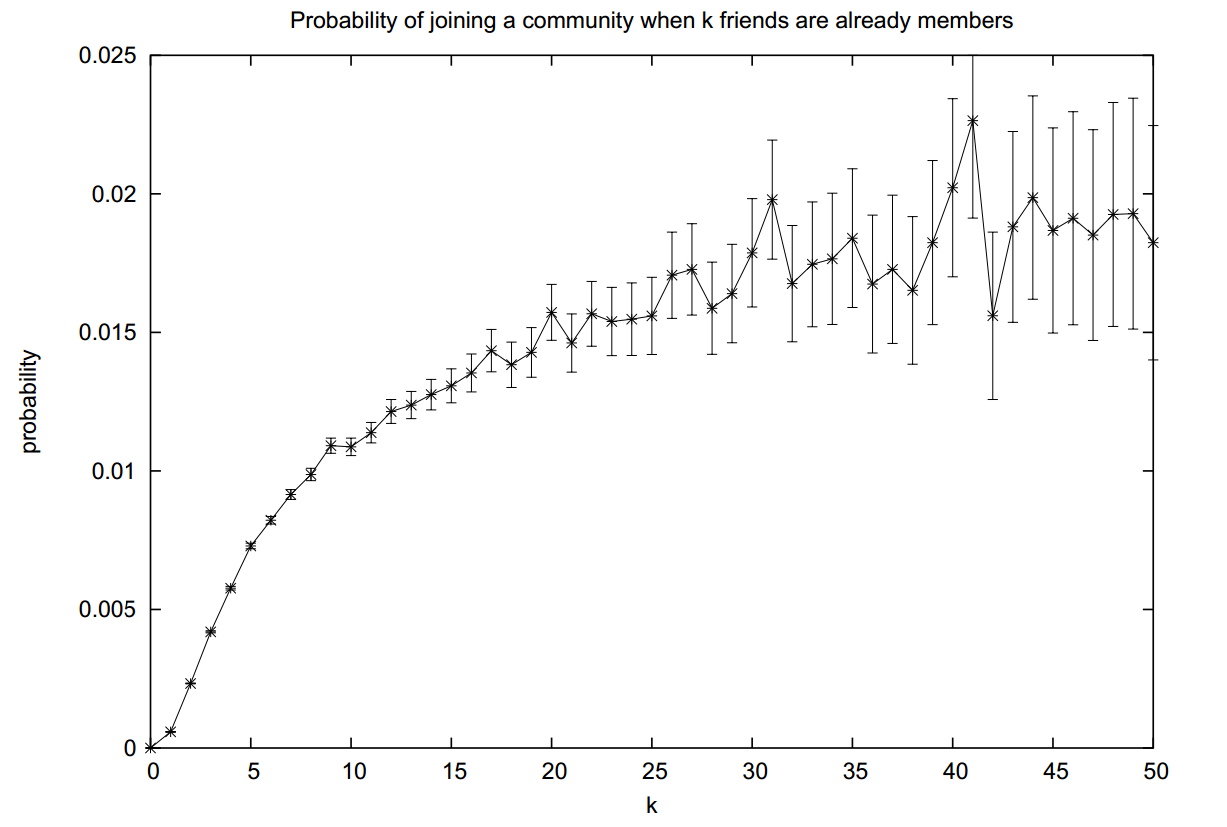
\includegraphics[width=0.8\textwidth]{LiveJounral.png}
	\caption{LiveJounral社区\cite{backstrom2006group}}\label{fig:LiveJounral}
\end{figure}
此外,杨洋\cite{yang2016role}等人观测了Flickr网络的情绪传播,把用户变开心的概率看做开心朋友数量的函数,
绘制的图片见原论文Figure 1(a),这里展示为图\ref{fig:Flickr}。
从图中可以看出整体上用户被影响的概率和朋友数量是一个超线性关系,也就是超模性质。
不同的用户阈值函数也不同,对于领导来说,阈值函数更偏向超模,而对普通用户阈值函数是次模的。
我们在后续的实验中也会采用这两种类似的$\varepsilon$-次模逼近函数设定。
\begin{figure}[h]
	\centering
	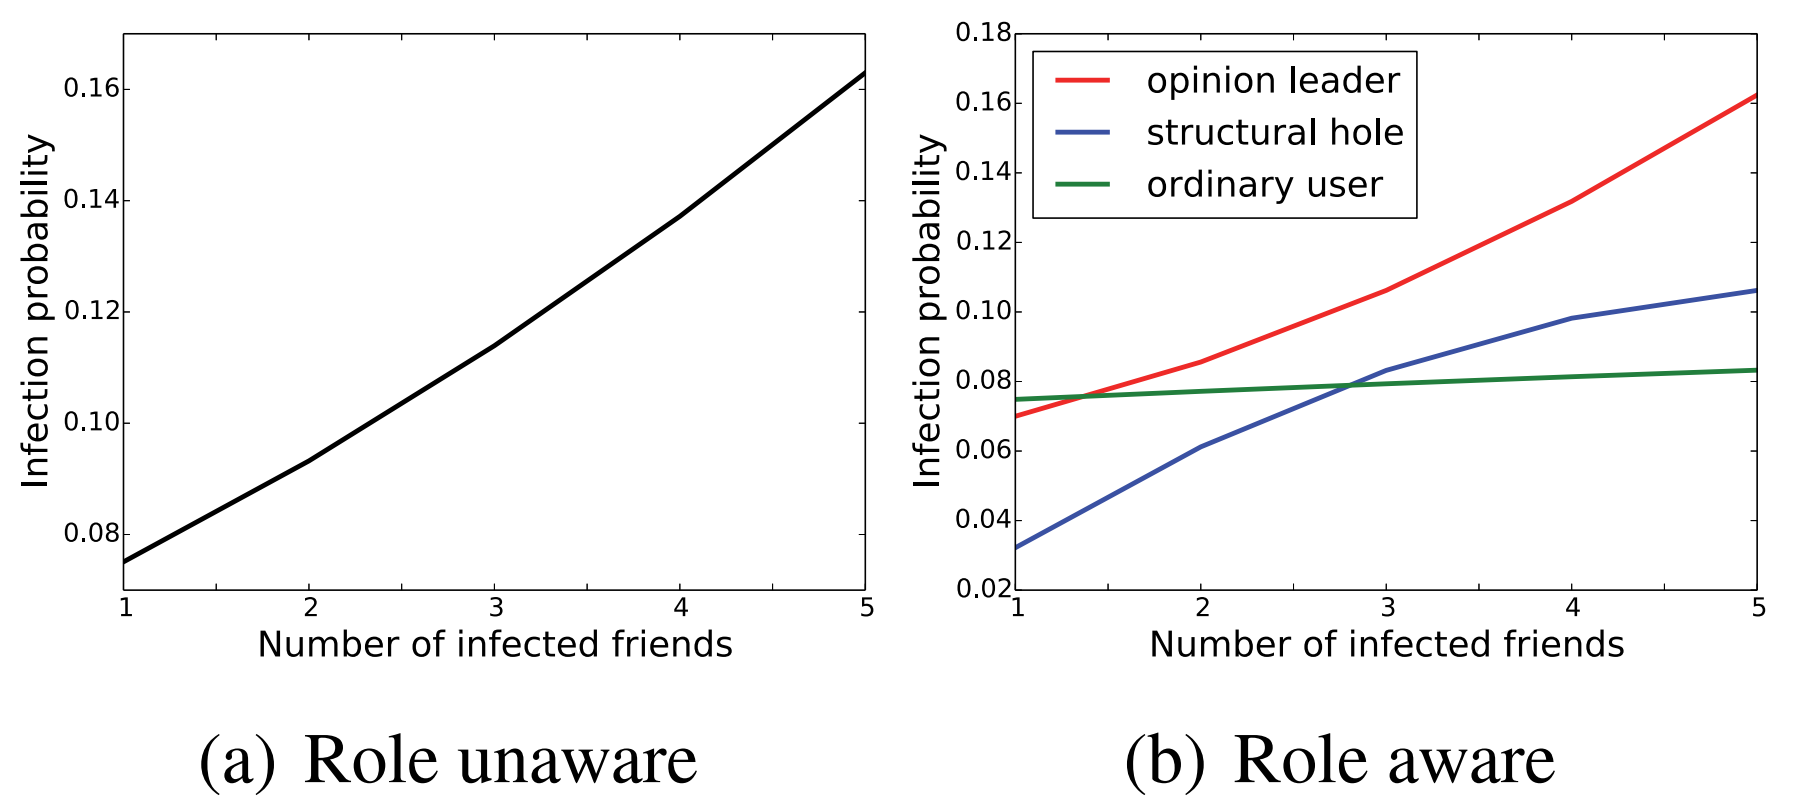
\includegraphics[width=0.8\textwidth]{Flickr.png}
	\caption{Flickr社区\cite{yang2016role}}\label{fig:Flickr}
\end{figure}

在给定$\varepsilon$-次模逼近函数定义和动机之后,我们介绍本文主要研究的问题。
本文主要研究图中有部分节点的阈值函数是$\varepsilon$-次模逼近函数的情况。
\begin{definition}[$(\gamma,\varepsilon)$-次模逼近图 ($(\gamma,\varepsilon)$-Almost Submodular Graph)]
给定参数$\gamma, \varepsilon \in (0,1)$,
一个$n$个节点的图如果至多有$n^{\gamma}$个节点阈值函数是$\varepsilon$-次模逼近,其余节点的阈值函数是次模的,
我们称其为是{\it $(\gamma,\varepsilon)$-次模逼近图}或者{\it $(\gamma,\varepsilon)$-次模逼近网络}。
\end{definition}
后续为了简便,阈值函数是$\varepsilon$-次模逼近的节点简写为{\it $\varepsilon$-次模逼近节点},
阈值函数是模的节点简写为{\it 次模节点},
$\varepsilon$-次模逼近可写作{\it $\varepsilon$-AS},
包含$\varepsilon$-次模逼近节点的图可写作{\it $\varepsilon$-次模逼近网络}。
$\gamma, \varepsilon$描述了图偏离次模的程度,$\gamma, \varepsilon$越大,图上影响力函数偏离次模越远。
接着,我们定义$(\gamma,\varepsilon)$-次模逼近图上的影响力最大化问题$(\gamma,\varepsilon)$-ASIM,也是本文研究的重点。

\begin{definition}[$(\gamma,\varepsilon)$-次模影响力最大化 ($(\gamma,\varepsilon)$-ASIM)]
给定一个$(\gamma,\varepsilon)$-次模逼近图和输入$k$,$(\gamma,\varepsilon)$-次模影响力最大化问题是
在这个有$n^{\gamma}$个$\varepsilon$-次模逼近节点节点的图上寻找影响力最大的,大小不超过$k$的种子集合。
\end{definition}


\section{$k$-激活函数}
接下来本节介绍$k$-激活函数。

\subsection{传染病模型}
$k$-激活本质上是用{\it 传染病}去模拟信息、疾病和想法在网络中的扩散。
网络中的节点都有三种状态:{\it 未激活}(inactive)、{\it 暴露}(exposed)和{\it 已激活}(activated)。
节点可以从未激活状态转变为状态,然后再进入激活状态,但是不能反方向转变,例如不能从已激活的状态变成未激活状态。

传染病传染的过程可以用离散的时间步骤$0,1,2,\ldots$来描述。
如果一个节点$u$在$t-1$时间有至少$k$个已经感染的邻居节点
(在有向图中指有$k$个已感染节点发出的有向边指向$u$),
那么在时间$t\ge 1$节点$u$就变为暴露状态,$k$是传染病的阈值。
一个已经暴露的节点可以立即或者在后续时间步骤中转变为感染状态,
这取决于传染病扩散的方式。
{\it 简单传染病}指$k=1$的传染病,也就是说$u$的一个已感染的邻居就可以让$u$变为感染状态(有可能感染$u$)。
而{\it 复杂传染病}则较难传染,因为复杂传染病的阈值$k \geq 2$,要感染一个新的节点,
至少需要两个已感染的邻居节点。
阈值$k\ge 2$的传染病称为$k$-复杂传染病。

对于$k$-复杂传染病来说,对应的阈值函数恰好是$k$-激活函数,$k$-激活函数的定义如下
\begin{definition}[$k$-激活]
对于一个定义在集合上的函数$f:2^V \to \mathbb{R}$,
如果对于$V$的任意元素个数小于$k$的子集$S \subseteq V:|S|<k$都有$f(S) = 0$,
并且任意元素个数不小于$k$的子集$S \subseteq V:|S|\geq k$都有$f(S) = 1$,
则称$f$为$k$-激活函数。
\end{definition}


本文主要研究传染病多快把整个网络都传染,这个可以用{\it 传播时间}来描述,
而在网络中的强连接和弱连接都固定后传播时间是定值。
传播时间是指从$k$个种子节点开始,整个网络都被感染时经过的时间步数。

\subsection{传染病模型下的路由}

本文主要研究了一种比较像分散式路由\cite{Kleinberg2000small}的扩散方式,
我们称之为{\it $k$-复杂传染病的路由}(简称{\it 复杂路由}),也称为{\it $k$-激活路由}。

在复杂路由中,最初会选择一个节点$t$作为目标,同时也有$k$个种子节点。
复杂路由的任务是尽快激活目标节点$t$,不同于传播过程的是,
每一个时间步骤中所有被暴露的节点不会被立即感染。
每一步,我们只能从暴露状态的节点集合中选择一个节点来感染。
选择节点的策略称为路由策略。
更进一步,当在时间$i$选择了节点$u$去感染时,算法仅仅知道已感染节点集合的所有邻居(在有向图中是已感染节点发出的有向边指向的节点)。
复杂路由在日常生活中的情景比较像一群人想要去影响一个目标,
但是无法直接影响到目标。
于是这群人逐渐的扩大自己的势力,拉拢他们认为可以对劝说目标有帮助的人入伙,最终影响到目标。
在扩大势力的时候,他们只知道已经入伙的人的朋友,而且拉拢入伙需要一定的代价,在每一步只能选择拉拢一个人。
注意到如果把$k$设置为$1$,
并且要求下一个被激活的节点是最新激活节点的邻居,这就是Kleinberg研究的分散式路由\cite{Kleinberg2000small}。

为了研究路由找到目标的速度,本文定义{\it $k$-激活路由时间}
为通过$k$-激活路由方式激活距离种子节点曼哈顿距离最远的目标节点$t$所需要的步骤。


\section{本章小结}
本章主要介绍了本文后续降采用的阈值函数和相关问题定义
3.1节介绍了$\varepsilon$-次模逼近函数和函数在现实生活中的意义,定义了$(\gamma,\varepsilon)$-次模影响力最大化问题。
3.2节介绍了$k$-激活函数和对应的复杂传染病模型,同时提供了离散路由的定义。

\chapter{$\varepsilon$-次模逼近网络的影响力最大化}

在$\varepsilon$-次模逼近网络中,一些节点的阈值函数是$\varepsilon$-次模逼近而不再是次模函数,整体的影响力函数也不再有次模性质。
本章中会先讨论$\varepsilon$-次模逼近节点的个数是图节点个数多项式的时影响力最大化的不可近似性,
然后又设计了$\varepsilon$-次模逼近节点较少时的近似算法。

\section{$(\gamma,\varepsilon)$-ASIM的不可近似性}
本节我们会证明对于$n$个节点的图中,即使只有有$n$的多项式个$\varepsilon$-次模节点,
影响力最大化问题也很难近似。
下文用定理给出这个不可近似性的精确描述,然后本节接下来的部分会证明这个定理。


\subsection{不可近似性的主要结论}
\begin{theorem}
\label{the:inapp}
对于任意的$\varepsilon \in (0,1)$和任意的$\gamma \in (0,1)$,
在$(\gamma,\varepsilon)$-次模逼近图上不存在近似比为$1 / n^{\frac{\gamma}{c}}$的影响力最大化近似算法,
除非P=NP,这里$c = 3+3/\log{\frac{2}{2-\varepsilon}}$。
\end{theorem}

这个定理说明了只要图中有$n^{\gamma}$个$\varepsilon$-次模节点,不管$\gamma$有多少,影响力最大化问题都不能被近似。
不可近似的程度正比于$\gamma$的大小,$\gamma$越大,影响力最大化问题越难被近似。
定力的证明基于机关(gadget)的构造,我们通过二叉树级联机关构造出一个概率与门(probabilistic-AND gate),
然后我们通过NP完全问题Set Cover的规约证明了不可近似比的下界。

\subsection{基于二叉树的概率与门}
本小节介绍概率与门的构造和计算与门成功的概率。先介绍基础的机关,然后介绍通过二叉树级联得到的概率与门,最后计算与门的概率。


\begin{figure}[htbp]
\centering
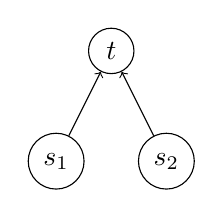
\begin{tikzpicture}[scale=0.7]
%\tikzstyle[thick]
\node at (1,2) [circle,draw](1) {$t$};
\node at (0,0) [circle,draw](2) {$s_1$};
\node at (2,0) [circle,draw](3) {$s_2$};
\path [->] (2) edge node{} (1);
\path [->] (3) edge node{} (1);
\end{tikzpicture}
\caption{基础机关结构}
\label{fig:gadget_basic}
\end{figure}
我们构建的机关如图\ref{fig:gadget_basic}所示,这个机关以节点$s_1,s_2$作为输入,以节点$t$作为输出。
节点$t$有两个入邻居,阈值函数$g(\cdot)$是$\varepsilon$-次模函数。
阈值函数$g(\cdot)$的赋值见等式\ref{eq:func_g}。
\begin{eqnarray*}
\label{eq:func_g}
g(S) =
\left\lbrace
\begin{aligned}
&0,		~ & |S|=0; \\
&\frac{1-\varepsilon}{2},	~ & |S|=1; \\
&1,		~ & |S|=2. \\
\end{aligned}
\right.
\end{eqnarray*}
函数$g(S)$的取值只依赖于输入集合的大小$|S|$,$g(\cdot)$被夹在两个线性的次模函数之间。
$g(\cdot)$自身是一个线性函数在$|S|=1$处向下偏移了$\varepsilon$。
这个基础机关距离与门的性质还很远,接下来我们介绍如何构造更复杂的机关。


我们希望构建出一个机关满足如下性质:
\begin{eqnarray*}
P_a(t) =
\left\lbrace
\begin{aligned}
&1,		~ & \mbox{$s_1,s_2$均被激活}; \\
&o(1),	~ & \mbox{$s_1,s_2$中只有一个被激活}; \\
&0,		~ & \mbox{$s_1,s_2$都未被激活}. \\
\end{aligned}
\right.
\end{eqnarray*}
其中$P_a(t)$是机关的输出节点$t$被激活的概率。
满足这样的性质,当输入节点$s_1,s_2$没有被全部激活时,输出节点$t$很大概率不会被激活。
前面的基础机关在$|S|=1$时,$t$被被激活的概率是$\frac{1-\varepsilon}{2}$,
我们做的就是通过二叉树级联机关放大$\frac{1-\varepsilon}{2}$和$\frac{1}{2}$的差距,
最终使得$|S|=1$时$t$很大概率不被激活,机关的构造如图\ref{fig:gadget_tree}所示。


\begin{figure}[htbp]
\centering
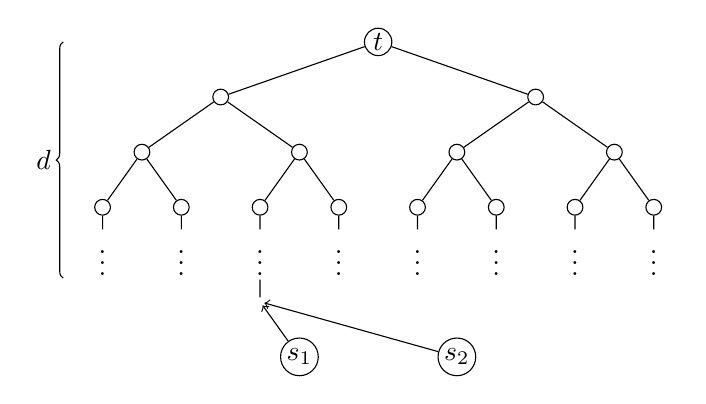
\begin{tikzpicture}[every node/.style={draw,circle,inner sep=1pt}]
% \draw[step=1cm, color=gray] (-5,-5) grid (5,5);
\tikzstyle{level 1}=[sibling distance=40mm,level distance=7mm]
\tikzstyle{level 2}=[sibling distance=20mm]
\tikzstyle{level 3}=[sibling distance=10mm]
\tikzstyle{level 4}=[level distance=6mm]
%\tikzstyle{level 5}=[sibling distance=15mm,level distance=10mm]
\draw[decorate, decoration={brace, mirror}] (-4cm, 0) -- (-4cm,-3cm);
\draw (-4.25cm, -1.5cm) node[draw=none] {$d$};

\node at (-1,-4) [circle,draw](2) {$s_1$};
\node at (1,-4) [circle,draw](3) {$s_2$};
\node {$t$}
	child{
		node{$~$}
		child{
			node{$~$}
			child{
				node{$~$}
				child{node[draw=none] {$\vdots$}
				}
			}
			child{
				node{$~$}
				child{node[draw=none]{$\vdots$}}
			}
		}
		child{
			node{$~$}
			child{
				node{$~$}
				child{node[draw=none]{$\vdots$}
					child{node[draw=none] (leaf_1) {$ $}}
				}
			}
			child{
				node{$~$}
				child{node[draw=none]{$\vdots$}
				}
			}
		}
	}
	child{
		node{$~$}
		child{
			node{$~$}
			child{
				node{$~$}
				child{node[draw=none]{$\vdots$}
				}
			}
			child{
				node{$~$}
				child{node[draw=none]{$\vdots$}}
			}
		}
		child{
			node{$~$}
			child{
				node{$~$}
				child{node[draw=none]{$\vdots$} }
			}
			child{
				node{$~$}
				child{node[draw=none] {$\vdots$}
					%child{node[draw=none] (leaf_2) {$ $}}
				}
			}
		}
	};

\path [->] (2) edge (leaf_1);
\path [->] (3) edge (leaf_1);
\end{tikzpicture}
\caption{二叉树机关$T_\varepsilon$}
\label{fig:gadget_tree}
\end{figure}

在这棵满二叉树中,输出节点$t$是二叉树的根节点,每个节点有一条有向边指向它的父节点。
对每个叶子结点$v$,输入节点$s_1,s_2$会发出有向边指向$v$。
二叉树中每个节点的阈值函数都是前文等式\ref{eq:func_g}定义的$\varepsilon$-次模函数$g(\cdot)$。
整个树状结构被定义为$T_\varepsilon$,$\varepsilon$就是函数$g(\cdot)$距离次模函数的偏移量。
二叉树的深度会在后文定义,我们用$v_i$表示深度为$i$的节点($t$的深度是$1$)。


很显然$s_1,s_2$都被激活时$P_a(t)=1$,$s_1$ or $s_2$都没有被激活时$P_a(t)=0$。
下面我们证明对于深度$d$的二叉树,$s_1,s_2$中只有一个被激活时,输出节点$t$被激活的概率是$O(2^{-d})$。
\begin{lemma}
\label{lem:tree_prob}
对于深度为$d$的机关$T_\varepsilon$,当输入节点只有一个被激活时,
输出节点$t$被激活的概率小于$(\frac{2-\varepsilon}{2})^{d}$。
\end{lemma}
\begin{proof}
对于所有的叶子结点$v_d$,可以得到$P_a(v_d) = \frac{1-\varepsilon}{2}$。
机关$T_\varepsilon$中同一层的节点之前激活与否是互相独立的。
给定一个基础机关(如图\ref{fig:gadget_basic}),如果每个输出节点被激活的概率都是$p$而且互相独立,则输出节点$t$被激活的概率是
\begin{equation*}
\begin{array}{ll}
& P_a(t) \\
= & p^2\times g(2) + 2p(1-p)\times g(1) + (1-p)^2\times g(0) \\
= & p^2 + 2p(1-p)\frac{1-\varepsilon}{2} = p(1-\varepsilon(1-p)).
\end{array}
\end{equation*}
根据这个公式,我们可以写出二叉树上不同深度节点被激活概率的递推公式。
\begin{equation}
\label{eq:recurrence}
P_a(v_i) = P_a(v_{i+1})(1-\varepsilon(1-P_a(v_{i+1}))) <  P_a(v_{i+1})(1-\varepsilon/2)
\end{equation}
不等号的成立是因为树的叶节点满足$P_a(v_d) = \frac{1-\varepsilon}{2}$,而且随着节点所处深度降低,被激活的概率递减。
所以对于树中的任意节点$v$都有$P_a(v) < \frac{1}{2}$。
根据递推公式\ref{eq:recurrence},输出节点$t$被激活的概率为
\begin{equation*}
\label{eq:p_a_t}
 P_a(t) 
=  P_a(v_1) 
<  \frac{1-\varepsilon}{2}(\frac{2-\varepsilon}{2})^{d-1} 
<  (\frac{2-\varepsilon}{2})^{d}.
\end{equation*}
节点$t$被激活的概率$P_a(t) = O(2^{-d})$,随着$d$的增加趋于$0$。
\end{proof}

由引理\ref{lem:tree_prob}我们知道$T_\varepsilon$在输入集合大小为$1$时输出节点被激活的概率是$o(1)$,
$T_\varepsilon$的确是一个两个输入节点的概率与门。
我们称概率与门在输入节点没有全部激活且输出节点保持未激活时为成功运作。


我们已经构造了两个输入节点的树状机关,我们拓展机关$T_\varepsilon$来得到$n$个输入节点的与门$T_\varepsilon^n$。
给定$n$个输入节点$s_1, s_2, \dots, s_n$,我们用节点$s_0$和$s_1$作为输入节点搭建$T_\varepsilon^n$,并令输出节点为$s_{12}$。
接下来可以把节点$s_{12}$和$s_{3}$作为输入节点搭建$T_\varepsilon^n$得到输出节点$s_{123}$。
以此类推,我们得到最终的输出节点$s_{12\dots n}$。
在这个结构中,$s_1, s_2, \dots, s_n$中有节点未被激活时,$s_{12\dots n}$很大概率不会被激活。
如果所有的$T_\varepsilon$都表现出与门的性质,那么整体上就构成了一个$n$个输入节点的概率与门。
由引理\ref{lem:tree_prob}可得深度为$d$的$T_\varepsilon$最多以$(\frac{2-\varepsilon}{2})^{d}$的概率不成功运作。
通过Union Bound,$T_\varepsilon^n$在输入中有未激活节点时输出节点被激活的概率至多为$n(\frac{2-\varepsilon}{2})^{d}$。
$T_\varepsilon^n$一共包含$n\times(2^d-1) = n2^d-n$个节点。



\subsection{基于Set Cover的不可近似性规约}
在本节基于概率与门,我们证明定理\ref{the:inapp}。
前面一节基于二叉树级联得到的2-输入概率与门$T_\varepsilon$,我们构造了$n$个输入的概率与门$T_\varepsilon^n$。
在接下来的证明中,我们说明如果$\varepsilon$-次模逼近网络中影响力最大化算法可以取得超过给定的近似比,那么Set Cover问题就可以在多项式时间内被解决。
证明的整体思路是对于集合覆盖的一个实例,我们构造一个网络。网络中代表元素的点是$T_\varepsilon^n$的输入,
然后把$T_\varepsilon^n$的输出点连接到数量很大的额外节点。
因此,当$k$个集合可以覆盖住所有元素时,额外节点都会被激活。否则,$T_\varepsilon^n$的输出大概率不会被激活,额外节点都未被激活。
\begin{proof}[定理\ref{the:inapp}证明]
我们考虑一个基于集合覆盖构建出的图,在这个网络中影响力最大化算法的近似比不能超过给定的值,否则集合覆盖问题就将被解决,这就导致矛盾。
令$e_1, e_2, \dots, e_n$为表示集合覆盖实例中$n$个元素的节点,$s_1, s_2, \dots, s_m$为表示$m$个集合的节点。
我们可以假定$m<n$,因为当$m\geq n$时,我们可以添加$m$个冗余节点(dummy nodes),他们分别被$m$个集合覆盖。
原始的集合覆盖有$k$个集合的解时,新的集合覆盖问题就有$m+k$个集合的解。
集合节点$s_i$会持有指向所有它覆盖元素节点的有向边,而且所有元素节点$e_j$的阈值函数是$f_{e_j}(1)=1$。
也就是说只要覆盖$e_j$的集合节点中至少有一个被激活,$e_j$就会被激活。
接下来们增加$n^\alpha$个与门节点$x_1, x_2, \dots, x_{n^\alpha}$,$\alpha$的值在后文确定。
在节点$x_k$和元素节点$e_1, e_2, \dots, e_n$之间插入$n$输入概率与门$T_\varepsilon^n$,$x_k$是输出节点,如图\ref{fig:inapp_structure}所示。
\begin{figure}[h]
	\centering
	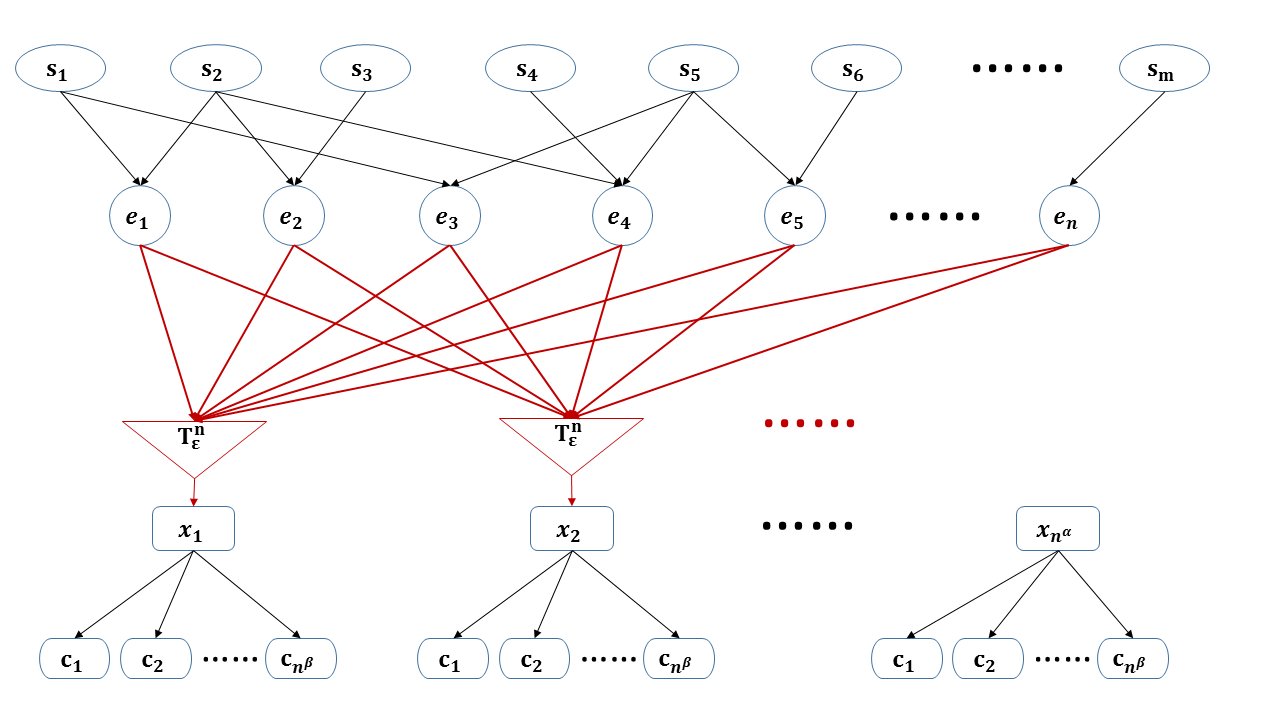
\includegraphics[width=\textwidth]{inapp_structure.png}
	\caption{集合覆盖构造$\varepsilon$-次模近似图}\label{fig:inapp_structure}
\end{figure}
然后对于参数$\alpha$,我们对每一个与门节点$x_k$添加$n^\alpha$个冗余节点$c_1, c_2, \dots, c_{n^\beta}$。
对每个冗余节点$c_l$,阈值函数同样是$f_{c_l}(1)=1$。
构建好的图中有集合节点$s_i$,元素节点$e_j$,与门节点$x_k$,冗余节点$c_l$以及构成概率与门的节点。
除了构成概率与门的节点阈值函数是等式\ref{eq:func_g}定义的$\varepsilon$-次模逼近函数,其余节点的阈值函数都是次模函数。
图\ref{fig:inapp_structure}中红色的边代表着概率与门中节点的阈值函数是$\varepsilon$-次模逼近函数。

接下来我们计算$T_\varepsilon^n$的深度,需要$T_\varepsilon^n$足够深才能以高概率保证$n^\alpha$个$T_\varepsilon^n$全部成功运作。
运行Union Bound,$n^\alpha$个$T_\varepsilon^n$至少有一个运作失败的概率至多是$n^{1+\alpha}(\frac{2-\varepsilon}{2})^{d}$。
令$d = (1+\alpha+\lambda)\log n / \log{\frac{2}{2-\varepsilon}}$,
在这个情况下所有概率与门$T_\varepsilon^n$均成功运作的概率至少是$1-n^{-\lambda}$。

如果我们能找到$k$个集合覆盖住所有$n$个元素,那么在这个构造的图中我们把对应那$k$个集合的节点选作种子节点。
接下来种子节点会激活所有的元素节点$e_1, e_2, \dots, e_n$,然后$T_\varepsilon^n$中的所有节点都会被激活。
最终,所有的与门节点$x_1, x_2, \dots, x_{n^\alpha}$以及他们指向的冗余节点都会被激活,一共被激活的节点个数是
$$k+n+n^{\alpha+1}(2^d-1)+n^{\alpha\beta} \geq n^{\alpha\beta}.$$
整个图中一共有
$$k+n+n^{\alpha+1}(2^d-1)+n^{\alpha\beta} \geq n^{\alpha\beta}$$
个节点,几乎图中所有的节点都会被激活。
另一方面,如果集合覆盖实例没有大小为$k$的解,就不能激活所有的元素节点$e_j$。
影响力传播过程中与门节点$x_1, x_2, \dots, x_{n^\alpha}$以高概率概率$1-n^{-\lambda}$都不会被激活。
此时,为了提升影响力,可以选择把与门节点$x_j$作为种子节点或者尽可能多的去激活元素节点$e_j$。
如果选择与门节点作为种子则最终激活至多$k+n+kn^{\beta}$个节点。
或者最多激活$n-1$个元素节点并激活几乎所有在概率与门机关中的$\varepsilon$-次模逼近节点,
这种情况下以高概率所有与门机关成功运作,最多$k+n-1+n^{\alpha+1}(2^d-1)$个节点会被激活。
如果概率与门运作失败,就假设此时所有节点最终都被激活。

现在我们设置参数$\alpha$和$\beta$,可以$\delta>0$取令$n^{\beta} = n^{\alpha-1} \cdot 2^d \cdot n^{\delta}$。
此时与门机关中节点的个数和冗余节点个数的比值为$n^{\alpha+1}(2^d-1) / n^{\alpha\beta} < n^{\frac{1}{\alpha-1}}$。
当$n$区域无穷时,如果集合覆盖问题无解,影响力范围以高概率$1-n^{-\lambda}$不会超过$kn^{\beta} \leq n^{\beta+1}$和$n^{\alpha+1}2^d$。
也就是说对于任意的影响力最大化算法,存在一个$N$个节点的图,其中至多有$n^{\alpha+1}(2^d-1)$个$\varepsilon$-次模逼近节点,
而对于算法输出的种子集合,以$1-n^{-\lambda}$的概率影响力不会超过$kn^{\beta} \leq n^{\beta+1}$和$n^{\alpha+1}2^d$,
除非集合覆盖问题有多项式时间的算法(NP=P)。
在这个图中,最优的种子集合$S^*$的影响力几乎是$N$,可以得到近似比不会超过
\begin{equation}
\label{eq:inapp_ratio}
\begin{array}{ll}
& \frac{\max\{kn^{\beta}, n^{\alpha+1}2^d\} * (1-n^{-\lambda}) + n^{-\lambda} * \sigma(S^*)}{\sigma(S^*)} \\
\leq & n^{-\lambda} + 
\frac{\max\{n^{\beta+1}, n^{\alpha+1}2^d\} * (1-n^{-\lambda})}
{k+n+n^{\alpha+1}(2^d-1)+n^{\alpha\beta} \geq n^{\alpha\beta}} \\
\leq & n^{-\lambda} + n^{-(\alpha-1)}
\end{array}
\end{equation}
这里$N \geq n^{\alpha+\beta}$,与门机关的深度为$d = (1+\alpha+\lambda)\log n / \log{\frac{2}{2-\varepsilon}}$,
参数$\beta = (\alpha+1) + (1+\alpha+\lambda) / \log{\frac{2}{2-\varepsilon}} + \delta$。
我们把参数带入不等式\ref{eq:inapp_ratio}和上述描述,得到
对于任意的$\alpha>1, \lambda>0, \delta>0$,存在$b = 1/\log{\frac{2}{2-\varepsilon}}$
$\varphi= \frac{ \min\{\alpha-1, \lambda\}}{2\alpha+\delta-1+b(1+\alpha+\lambda)}$和
$\gamma =\frac{\alpha+1+b(1+\alpha+\lambda)}{2\alpha+\delta-1+b(1+\alpha+\lambda)}$,
任意的基于$(\gamma,\varepsilon)$-次模逼近图的影响力最大化算法,
都可以构造出一个$\varepsilon$-次模逼近图实例,在这个图上算法的近似比不会超过$n^{-\gamma}$。
注意到这里$\varphi \geq \frac{\gamma}{3+3b}$在我们设定 $\alpha=\lambda+1$且$\lambda \geq 1$时。
$\gamma$的取值范围是$(0,1)$,也就是对于任意比例的$\varepsilon$-次模逼近节点结论都成立。
至此,我们证明了定理\ref{the:inapp}。
\end{proof}

\section{基于上下届的近似算法}
在前一小节,我们证明了$\varepsilon$-次模逼近节点较多时影响力最大化算法很难近似。
在本小姐,我们讨论图中只有比较少的$\varepsilon$-次模逼近节点的情况,通常是常数个或者$\log n$个。
首先我们提供了基于图中有较少非次模节点的朴素的贪心算法,
然后把非次模节点的阈值函数限定为$\varepsilon$-次模逼近并进一步提升了算法效果。


\subsection{非次模节点较少图的近似算法}
对于有$\ell (\ell<k)$个非次模节点的图,我们提供如下的近似算法。
\begin{algorithm}[h]
	\caption{\textbf{Naive-Greedy(G,k)}: Greedy for graph with $\ell$ non-submodular nodes.}
	\label{alg:naive_greed} 
	\begin{algorithmic}[1]
		\Require $G$: social graph of general threshold model, $k$: budget of seeds.
		\Ensure selected seed set $S$.
		\State Initialize $S = \emptyset$
		\ForAll { non-submodular node $v$}
			\State $S = S \cup \{v\}$
		\EndFor
		\For {$i=1$ to $k - \ell$}
			\State $v = \mathrm{argmax}_{u \in V \setminus S}$ \Call{MC-Spread}{$S \cup \{u\}, G$}
			\State $S = S \cup \{u\}$
		\EndFor
		\State \Return $S$
	\end{algorithmic} 
\end{algorithm}
在Algorithm\ref{alg:naive_greed}中,首先把所有的非次模节点加入种子集合,然后再依据贪心策略添加余下的$k - \ell$节点。
接下来分析算法的性能:


\begin{theorem}\label{the:naive_greedy}
给定一个$n$个节点的图$G$,其中除了$\ell < k$个节点的阈值函数是非次模函数,其余节点的阈值函数均是次模。
在图$G$上的影响力最大化算法Algorithm\ref{alg:naive_greed}可以取得$(1-e^{-\frac{k-\ell}{k}})(1-\frac{1}{e})$的近似比。
\end{theorem}
\begin{proof}
假设$S^*$是图$G$影响力最大化的最优种子集合,$V_e$是$\ell$个阈值函数非次模的节点集合,
令$S^*_{V_e} = S^* \cup V_e$。
很显然,由于影响力函数$\sigma(\cdot)$是单调非减的$\sigma(S^*_{V_e}) \geq \sigma(S^*)$。
由于$V_e$中的节点阈值函数是非次模的,所以我们不能直接应用贪心策略去做。
但是把$V_e$加入到种子节点后,函数$\sigma(S\cup V_e)$对于输入$S \subseteq V-V_e$来说是满足次模性质的。

通过预先把$V_e$中的节点加入种子集合,然后再通过贪心策略添加$k$个种子得到一个大小为$k+\ell$的种子集合$S^g_{V_e,k}$。
贪心策略有$1-\frac{1}{e}$的近似比,所以$\sigma(S^g_{V_e,k}) \geq (1-\frac{1}{e})\sigma(S^*_{V_e})$。
我们假设$S^*_{V_e}=V_e \cup \{s_1,s_2,\dots,s_{k'}\}, k'\leq k$, 其中$s_i \not\in V_e$是不属于$V_e$的节点。
令$S_i = \{s_1,s_2,\dots,s_i\}$。
实际上,根据$1-1/e$近似比的证明过程,对于$i\leq k$我们有:
\begin{equation}
\label{eq:1e_proof}
\begin{array}{ll}
&\sigma(S^*_{V_e})\\
\leq & \sigma(S^*_{V_e} \cup S^g_{V_e,i})\\
= & \sigma(S^g_{V_e,i}) +
	\sum_{j=1}^{k'} \big( \sigma(S^g_{V_e,i} \cup S_j) - 	
	\sigma(S^g_{V_e,i} \cup S_{j-1})\big)\\
\leq & \sigma(S^g_{V_e,i}) +
	\sum_{j=1}^{k'} \big( \sigma(S^g_{V_e,i} \cup \{s_j\}) - 	
	\sigma(S^g_{V_e,i})\big)\\
\leq & \sigma(S^g_{V_e,i}) +
	k\cdot \big( \sigma(S^g_{V_e,i+1})-\sigma(S^g_{V_e,i})\big)\\
\end{array}
\end{equation}
不等式\ref{eq:1e_proof}的第一行是因为影响力函数$\sigma$是单调非减的,
第三行是因为$\sigma$是次模函数。
不等式\ref{eq:1e_proof}第四行成立的原因是$S^g_{V_e,i+1}$是基于贪心算法
在$S^g_{V_e,i}$的基础上选出的边际影响力最大的节点,边际影响力要大于节点$s_{i+1}$。
然后我们可以得到:
\begin{equation*}
\label{eq:sub_greedy_re}
\begin{array}{ll}
\sigma(S^*_{V_e}) - \sigma(S^g_{V_e,i}) \leq
k\cdot \big( \sigma(S^g_{V_e,i+1})-\sigma(S^g_{V_e,i})\big) \\
\sigma(S^*_{V_e}) - \sigma(S^g_{V_e,i+1}) \leq
(1-\frac{1}{k}) \big( \sigma(S^*_{V_e}) - \sigma(S^g_{V_e,i}) \big)
\end{array}
\end{equation*}
如果只使用贪心策略选择$k-\ell$个节点的话,
\begin{equation*}
\begin{array}{ll}
& \sigma(S^*_{V_e}) - \sigma(S^g_{V_e,k-\ell}) \\
\leq & (1-\frac{1}{k})^{k-\ell} (\sigma(S^*_{V_e}) - \sigma(V_e))\\
\leq & (1-\frac{1}{k})^{k-\ell} \sigma(S^*_{V_e})
\end{array}
\end{equation*}
公司的第二行是重复使用不等式\ref{eq:sub_greedy_re}。
所以在种子集合加入$V_e$后再选择$k-\ell$个种子的情况下,
$$\sigma(S^g_{V_e,k-\ell})
\geq (1-(1-\frac{1}{k})^{k-\ell}) \sigma(S^*_{V_e})
\geq (1-e^{-\frac{k-\ell}{k}}) \sigma(S^*)$$

所以先把非次模节点加入种子集合,然后再贪心的选择$k-\ell$个种子节点,依然可以得到一个近似比$(1-e^{-\frac{k-\ell}{k}})$的解,定理证明完毕。
\end{proof}

Algorithm\ref{alg:naive_greed}有一定局限性,非次模节点个数不能太多,不能超过给定的$k$。
然后算法也只能粗暴的把非次模节点加入种子集合来保证次模性质,非次模节点个数较多时算法近似比很差。
同时算法对于非次模节点的阈值函数没有限制,在阈值函数是$\varepsilon$-次模时不能提升效果。

\subsection{基于次模上下界的近似算法}
在前一小节,本文提供了一个简单的针对图中有$\ell~(\ell<k)$个非次模节点的影响力最大化近似算法。
在本节,我们考虑非次模函数是$\varepsilon$-次模逼近函数的情况,提供了一个基于$\varepsilon$-次模逼近图的近似算法,并证明了算法的近似比。
整体思路是概率空间的映射。

在定义\ref{def:eas}中,我们定义了$\varepsilon$-次模逼近函数$f_v$的次模上界函数$\overline{f}_v$和次模下界函数$\underline{f}_v$。
注意到次模函数也是$\varepsilon$-次模逼近,对次模函数$f_v$来说,$\underline{f}_v = f = (1-\varepsilon)\overline{f}_v$。
根据定义,可以推出对于任意的输入$\underline{f}_v \geq (1-\varepsilon)\overline{f}_v$。
给定一个包含$\varepsilon$-次模逼近节点的图,我们可以把每个节点的阈值函数替换成次模下界函数,
然后在新构建的图上运行经典的基于次模的影响力最大化算法(Algorithm~\ref{alg:Galg_L})。
下面的定理证明了这种贪心算法的近似比。

\begin{algorithm}[h]
	\caption{\textbf{Galg-L($G,k,\mathcal{A},\{\overline{f}_v\},\{\underline{f}_v\}$)}: algorithm for zoomed threshold model.}
	\label{alg:Galg_L} 
	\begin{algorithmic}[1]
		\Require $G$: social graph, $k$: budget of seeds, $\mathcal{A}$: greedy IM algorithm, 
			$\{\overline{f}_v\},\{\underline{f}_v\}$: submodular upper and lower function.
		\Ensure selected seed set $S$.
		\State Initialize $S = \emptyset$
		\State replace each nodes $v$'s threshold function $f_v$ with $\underline{f}_v$
		\State run greedy algorithm $\mathcal{A}$ on $G$ with $\{\underline{f}_v\}$ and obtain $S$
		\State \Return $S$
	\end{algorithmic} 
\end{algorithm}


\begin{theorem}
\label{thm:app_alg}
给定通用阈值模型的一个图$G$,
如果图中只有$c$个节点的阈值函数是$\varepsilon$-次模逼近而其余节点的阈值函数均是次模,
那么算法{\bf Galg-L}可以输出近似比为$(1-\frac{1}{e})(1-\varepsilon)^c$的种子集合。
\end{theorem}
\begin{proof}
令$V_e$为$\varepsilon$-次模逼近节点的集合。
不失一般性,我们可以假设$V_e = \{v_1,v_2,\dots,v_c\}$。
现在考虑这两个阈值函数均为次模函数的图$\overline{G}, \underline{G}$,它们的节点和图$G$一致.
这两个图中每个节点$v$的阈值函数分别是$\overline{f}_v$和$\underline{f}_v$。
图$G$、$\overline{G}$和$\underline{G}$中,$V-V_e$内的节点阈值函数相同,
$V_e$内节点的阈值函数分别为$\varepsilon$-次模逼近、次模上界和次模下界函数。

对于通用阈值模型来说,如果每个节点$v$的阈值$\theta_v$都被确定了,传播过程就变成了确定性的。
一个阈值函数为$\{f_v\}$的图$G$和给定的节点阈值$\{\theta_v\}$被称为{\it 可能世界图}(possible world),
这和独立级联模型的活边子图(live-edge graph)很类似。
一个可能世界图可以被表示为
$$\{\theta_{v_1},\theta_{v_2},\dots,\theta_{v_n};f_{v_1},f_{v_2},\dots,f_{v_n}\}$$
分别是每个节点的阈值和阈值函数。
这里我们通过$\theta_{v}\leq 1-\varepsilon (v\in V_e)$构建$\underline{G}$和$\overline{G}$之间可能世界图的一一映射。

\begin{equation}
\label{eq:possible_world}
\begin{array}{ll}
\{\theta_{v_1},\dots,\theta_{v_c},\theta_{v_{c+1}}\dots,\theta_{v_n};
f_{v_1}, \dots,f_{v_n}\} \leftrightarrow \\
\{\frac{\theta_{v_1}}{1-\varepsilon},\dots,\frac{\theta_{v_1}}{1-\varepsilon},\theta_{v_{c+1}}\dots,\theta_{v_n};
\frac{f_{v_1}}{1-\varepsilon},\dots,\frac{f_{v_c}}{1-\varepsilon},f_{v_{c+1}},\dots,f_{v_n}\} \\
\end{array}
\end{equation}

等式\ref{eq:possible_world}描述了$\underline{G}$和$\overline{G}$的一一映射。
给定$\underline{G}$的任意可能世界图,
对于任意在$V_e$中的节点$v\in V_e$且阈值$\theta_{v}\leq 1-\varepsilon$,
把阈值$\theta_{v}$放大至$\frac{\theta_{v}}{1-\varepsilon}$。
与此同时,也把这些节点的阈值函数也放大$\frac{1}{1-\varepsilon}$倍到$\frac{f_{v}}{1-\varepsilon}$。
显然,这个放大过程不会影响在可能世界图中的传播过程,
但是放大之后$\underline{G}$的可能世界图变成了$\overline{G}$中的一个可能世界。

期望的影响力$\sigma$可以通过对阈值积分计算:
$$\sigma(S)=\int_{\mathbb{\theta}\in[0,1]^n} \mathcal{D}(\mathbb{\theta};f,S) \mbox{d}_{\mathbb{\theta}}$$
$\mathcal{D}(\mathbb{\theta};f,S)$代表的是在可能世界图$(\mathbb{\theta};f)$中种子集合$S$确定的的影响力大小。
称图$\overline{G},\underline{G}$的影响力函数分别为$\overline{\sigma},\underline{\sigma}$。
定义$\vec{\theta}\in[0,1]^n$为$n$个节点阈值组成的$n$维向量,
$\vec{\theta}_e \in[0,1]^{c}$和$\vec{\theta}'\in[0,1]^{n-c}$分别是集合$V_e$和$V-V_e$的阈值向量。
类似的可以定义阈值函数向量,定义$V_e$和$V-V_e$的阈值函数向量分别为$\vec{f}_e,\vec{f}'$。
一个可能世界图被简写为:
$$\{\vec{\theta}_e,\vec{\theta}';\vec{f}_e,\vec{f}'\}$$
对于任意的种子集合,可以得到:
\begin{equation}
\label{eq:sigma_geq}
\begin{array}{ll}
&\underline{\sigma}(S)\\
=&\int_{\vec{\theta}\in[0,1]^n} \mathcal{D}(\vec{\theta};\vec{f},S) \mbox{d}_{\vec{\theta}} \\
\geq&\int_{\vec{\theta}_e\in[0,1-\varepsilon]^c}\int_{\vec{\theta}'\in[0,1]^{n-c}} \mathcal{D}(\vec{\theta}_e,\vec{\theta}';\vec{f},S) \mbox{d}_{\vec{\theta}_e}\mbox{d}_{\vec{\theta}'} \\
=&(1-\varepsilon)^c \int_{\frac{\vec{\theta}_e}{1-\varepsilon}\in[0,1]^c}\int_{\vec{\theta}'\in[0,1]^{n-c}} \mathcal{D}(\vec{\theta}_e,\vec{\theta}';\vec{f},S) \mbox{d}_{\frac{\vec{\theta}_e}{1-\varepsilon}}\mbox{d}_{\vec{\theta}'} \\
=&(1-\varepsilon)^c \int_{\frac{\vec{\theta}_e}{1-\varepsilon}\in[0,1]^c}\int_{\vec{\theta}'\in[0,1]^{n-c}} \mathcal{D}(\frac{\vec{\theta}_e}{1-\varepsilon},\vec{\theta}';\frac{\vec{f}_e}{1-\varepsilon},\vec{f}',S) \mbox{d}_{\frac{\vec{\theta}_e}{1-\varepsilon}}\mbox{d}_{\vec{\theta}'} \\
=&(1-\varepsilon)^c \int_{\vec{\theta}\in[0,1]^n} \mathcal{D}(\vec{\theta};\frac{\vec{f}_e}{1-\varepsilon},\vec{f}',S) \mbox{d}_{\vec{\theta}} \\
=&(1-\varepsilon)^c \overline{\sigma}(S).\\
\end{array}
\end{equation}
不等式\ref{eq:sigma_geq}的第三个等号利用了$\underline{G}$和$\overline{G}$可能世界图的一一映射。
因此,给定一个种子集合$S$,在图$\overline{G}$和图$\underline{G}$中对应的影响力函数满足关系:
$$\underline{\sigma}(S) \geq (1-\varepsilon)^c \overline{\sigma}$$



称$\sigma$为原图$G$的影响力函数,令$\overline{S}^*,S^*,\underline{S}^*$分别代表
$\overline{\sigma}, \sigma, \underline{\sigma}$的影响力最大化问题最优解。
显然$\overline{\sigma}(\overline{S}^*) \geq \sigma(S^*)$,因为对任意节点$v$都有$\overline{f}_v \geq f_v$。
根据前文的不等式\ref{eq:sigma_geq},推出
$$\underline{\sigma}(\underline{S}^*)
\geq \underline{\sigma}(\overline{S}^*)
\geq (1-\varepsilon)^c \overline{\sigma}(\overline{S}^*)$$
因此对于基于$\overline{\sigma}$的贪心算法$\mathcal{A}$的输出种子集合$S^{\mathcal{A}}$,有近似比如下:
\begin{equation*}
\begin{array}{ll}
& \sigma(S^{\mathcal{A}}) \\
\geq & \underline{\sigma}(S^{\mathcal{A}}) \\
\geq & (1-\frac{1}{e})\underline{\sigma}(\underline{S}^*)\\
\geq & (1-\frac{1}{e})(1-\varepsilon)^c \overline{\sigma}(\overline{S}^*) \\
\geq &(1-\frac{1}{e})(1-\varepsilon)^c \sigma(S^*) \\
\end{array}
\end{equation*}
至此定理证明完毕。
\end{proof}

如果Algorithm~\ref{alg:Galg_L}$\varepsilon$-次模逼近函数替换成对应的上界然后运行贪心算法,
可以得到类似的结果,近似比也是$(1-\frac{1}{e})(1-\varepsilon)^c$,我们称这种算法为\textbf{Galg-L}。
证明过程中用到的技巧和Lu等人\cite{lu2015competition}的{\em sandwich approximation}有些相似。
但是他们的近似比依赖于尚未确定的影响力大小,而我们的工作利用概率空间映射直接求出了近似比的数值。


\section{本章小结}
本章主要讨论了$\varepsilon$-次模逼近网络中影响力最大化问题,
给出了图中有$n$的多项式个$\varepsilon$-次模逼近节点时的不可近似性,
最后针对图中较少$\varepsilon$-次模逼近的情况分别基于贪心策略和概率空间映射策略设计了两个近似算法,各自分析了近似比。
4.1节分析讨论了$n$个节点的图中有$n^{\gamma}$个$\varepsilon$-次模逼近节点的情况,基于机关构造从NP完全问题集合覆盖给出了不可近似性证明的规约。
4.2节首先给出针对图中有常数个非次模节点的近似算法,然后基于$\varepsilon$-次模逼近函数的次模上下界设计了近似算法,通过概率空间映射给出近似比证明。








%\chapter{总结与展望}
\section{研究工作总结}
信息化社会的到来,社交网络的用户量在爆发式增长。
社交网络中信息的扩散机制和基于社交网络的营销策略越发成为研究热点。
在本文中,我们研究学习了社交网络中一些非次模的问题,主要是基于非次模的阈值函数。
之前的研究大多集中在次模阈值函数和次模影响力函数,我们的研究和他们大不相同。
根据前人的实验观察,我们研究了两类非次模函数----$\varepsilon$-次模逼近函数和$k$-激活函数,
然后分别讨论了基于$\varepsilon$-次模逼近函数的影响力最大化问题和基于$k$-激活函数的小世界网络路由问题。
首先我们证明了尽管$\varepsilon$-次模逼近函数和次模函数很接近,
在有$\varepsilon$-次模逼近节点的图中影响力最大化问题依然很难近似。
通过构造概率与门并从NP完全问题集合覆盖归约,我们证明了
$n$个节点的图中只要有$n$的多项式个$\varepsilon$-次模逼近节点影响力最大化算法就无法做到$log$近似。
然后我们通过把$\varepsilon$-次模逼近函数替换成次模的上界或者下界,转化问一个次模优化问题,
设计了近似算法\textsf{Galg-U}和\textsf{Galg-L}。
基于概率空间映射,我们证明了这个近似算法的近似比为$(1-\frac{1}{e})(1-\varepsilon)^c$,
其中$c$是$\varepsilon$-次模逼近节点的个数。
接下来我们研究了Kleinberg小世界网络中,基于$k$-激活函数的路由。
本文定量地研究了从两个相邻的种子节点开始去感染一个网格上最远目标$t$需要的步数,也就是路由时间。
在每一步,只有一个节点会被激活,选择被激活节点的策略是分散式的,也就是路由选择策略只能基于当前被激活的节点发出的强连接和弱连接。
复杂路由比较像社交网站上最近提出的一个应用:主动交友,主动交友是指在像Facebook、人人网等社交网站上通过添加一些中间好友来增加目标接受自己好友请求的概率\cite{YangHLC13}。
本文指出与$k$-激活传播不同,对于所有的$\alpha$,$k$-激活路由时间均有$n$的多项式的下界,即使每一步允许激活多个节点。


本文的最后实现了算法\textsf{Galg-U}和\textsf{Galg-L}和其他基准算法,
并且在真实的社交网络{\em NetHEPT}、{\em Flixster}和{\em DBLP}上测试对比了算法和其他基准算法效果。
在小数据集上,\textsf{Galg-U}和\textsf{Galg-L}算法效果比\textsf{Greedy}稍好,
但是算法的运行时间要少很多,因为\textsf{Galg-U}和\textsf{Galg-L}可以利用一些次模上下界利用\textsf{TIM}算法加速。
在较大的网络{\em Flixster}和{\em DBLP}上,\textsf{Galg-U}和\textsf{Galg-L}均比其他基准算法要好。
而且在$\varepsilon$-次模逼近节点个数达到总结点个数$\frac{1}{3}$时,算法的表现依然很好。
这说明\textsf{Galg-U}和\textsf{Galg-L}不仅仅有理论近似比保证,实际中运行效果也很好。




\section{未来工作的展望}
在影响力最大化问题上,本文目前的研究主要集中在$\varepsilon$-次模逼近函数,
但是对于那些和次模函数相距很远的非次模阈值函数,我们还不知道如何设计有效的算法。
此外,我们提出的算法在实验中采用了逆向可达集合进行加速。
并不是所有的次模函数都可以使用逆向可达集合,
研究哪些函数可以使用逆向可达集合进行加速或者设计基于次模函数的加速算法也是新的研究方向。

其次,在研究$k$-激活路由时,为了更好地应用延迟选择原则,本文采用了有向Kleinberg小世界网络模型。
因为每个节点的弱连接平均数量仍为常数,有向小世界网络和无向小世界网络中$k$-激活路由的效率应该不会相差太多。
后续的工作希望可以研究$k$-激活路由在无向Kleinberg小世界网络中的性能。
未来也可以研究在什么样结构的网络中$k$-激活路由可以很快找到目标,探讨$k$-激活路由在其他小世界模型中的执行效率。
为$k$-激活路由寻找更广泛的应用场景也是未来需要进行的工作之一。



%\ICTbackmatter{\bibliography{bib/ref}\nocite{*}}
\ICTbackmatter{\bibliography{bib/ref}}
%\bibliography{bib/ref}
%
\begin{thanks}


在完成硕士学位论文之际,我在此向所有支持我、关心我的老师、师兄、同学和家人致以最衷心的感谢。
是你们的帮助,让我能够顺利完成毕业设计。
感谢中科院计算所前瞻实验室所对我的支持,感谢算法与复杂性课题组,
让我能够在一个科研环境优越的地方研究学习。


首先十分感谢我的指导教师孙晓明研究员。
自从我研一进入实验室以来,孙老师在科研、学习、生活方面给了我非常多的帮助。
感谢孙老师对我论文的选题、设计、完成以及论文修改等各个方面给予的悉心指导。
我也要感谢答辩组的各位老师,卜东波老师、和张家琳老师,你们在开题答辩和中期检查时都给提出了我非常重要的指导意见,
让我对自己的工作有了更深刻的认识,得到了新的启示。

我还要感谢在微软亚洲研究院实习时对我科研进行过指导的陈卫老师,
每周和你的讨论我都收益颇多,你对我在科研部分给予了细致的指导,在这里衷心地感谢你对我的教导。


感谢我的好朋友曾钢同学,毕设过程中我们互相鼓励,谢谢你的一路支持。
也感谢我的舍友顾茂杰和朱良昌以及实验室的岑武斌同学,是你们陪伴我走过了毕设的日子,谢谢你们对我的鼓励和支持。
我还要感谢实验室的师兄师姐们,感谢你们对我毕业设计提出了宝贵的意见,耐心的解答我们的疑惑。

在此,也要感谢我的家人对我的支持和鼓励,特别是父亲和母亲,你们的鼓励永远让我充满动力。

最后要感谢我的女朋友,在研究生阶段,让我踏实安心的工作,默默地支持我,谢谢你一直以来的陪伴!


感谢所有给予过我帮助与支持的老师同学们!


\end{thanks}

%
\begin{resume}

\begin{resumelist*}{教育经历}
\resumelistitem 2009年9月---~2013年7月,武汉大学,计算机学院,学士
\resumelistitem 2013年9月---~2016年7月,中国科学院,计算技术研究所,硕士
\end{resumelist*}

\begin{resumelist}{【攻读硕士学位期间发表的论文】}
\resumelistitem Jingya Tang, Dongming Zhang, Yongdong Zhang, Qi Tian, Region Similarity Arrangement for Image Retrieval. IEEE International Conference on Multimedia and Expo (ICME), IEEE, 2016. 
\end{resumelist}

\begin{resumelist}{【攻读硕士学位期间参加的科研项目】}

\resumelistitem 大规模图像检索系统(国家高新技术研究与发展计划)
\resumelistitem 基于区域相似性的大规模图像检索的研究 
\resumelistitem 基于深度卷积网络的民族服饰检测的研究

\end{resumelist}

\end{resume}

\end{document}
